% !TEX encoding = UTF-8 Unicode
% !TEX root = ../Saunkin.tex

\chapter{Implementation} \label{c3:implementation}

The system implements the citation analysis described in Section~\ref{sec:methodology}.
It takes an author name as input and returns citation counts, broken down into direct, co-author or external citations.
This chapter describes the component structure, data handling and processing steps to produce the results.

\section{System overview} \label{sec:system-overview}

There are two major use cases that the system attempts to satisfy.

\begin{description}
    \item[Author identification.] Select the unique author, whose citations user wants to examine.

    The initial search returns profiles matching the name provided.
    As the results can contain multiple entries matching the name, each item includes affiliations where available from the data source, or the user can request a list of publications, to help identify a particular author.

    The profiles are grouped by provider, as each source does not guarantee to use identifiers compatible with other sources.
    Matching a profile from one source to a profile from another would require a new algorithm to match identities, which is out of scope for this work.

    \item[Citation classification.] Having selected an author, collect all publications and incoming citations, classify them into the groups, to produce the aggregate counts.
    The backend compares author lists of each citing paper to classify citations according to the algorithm from Section~\ref{sec:methodology}.
    The results returned to the frontend contain counts and raw data.
\end{description}


\begin{figure}[tb]
    \centering
    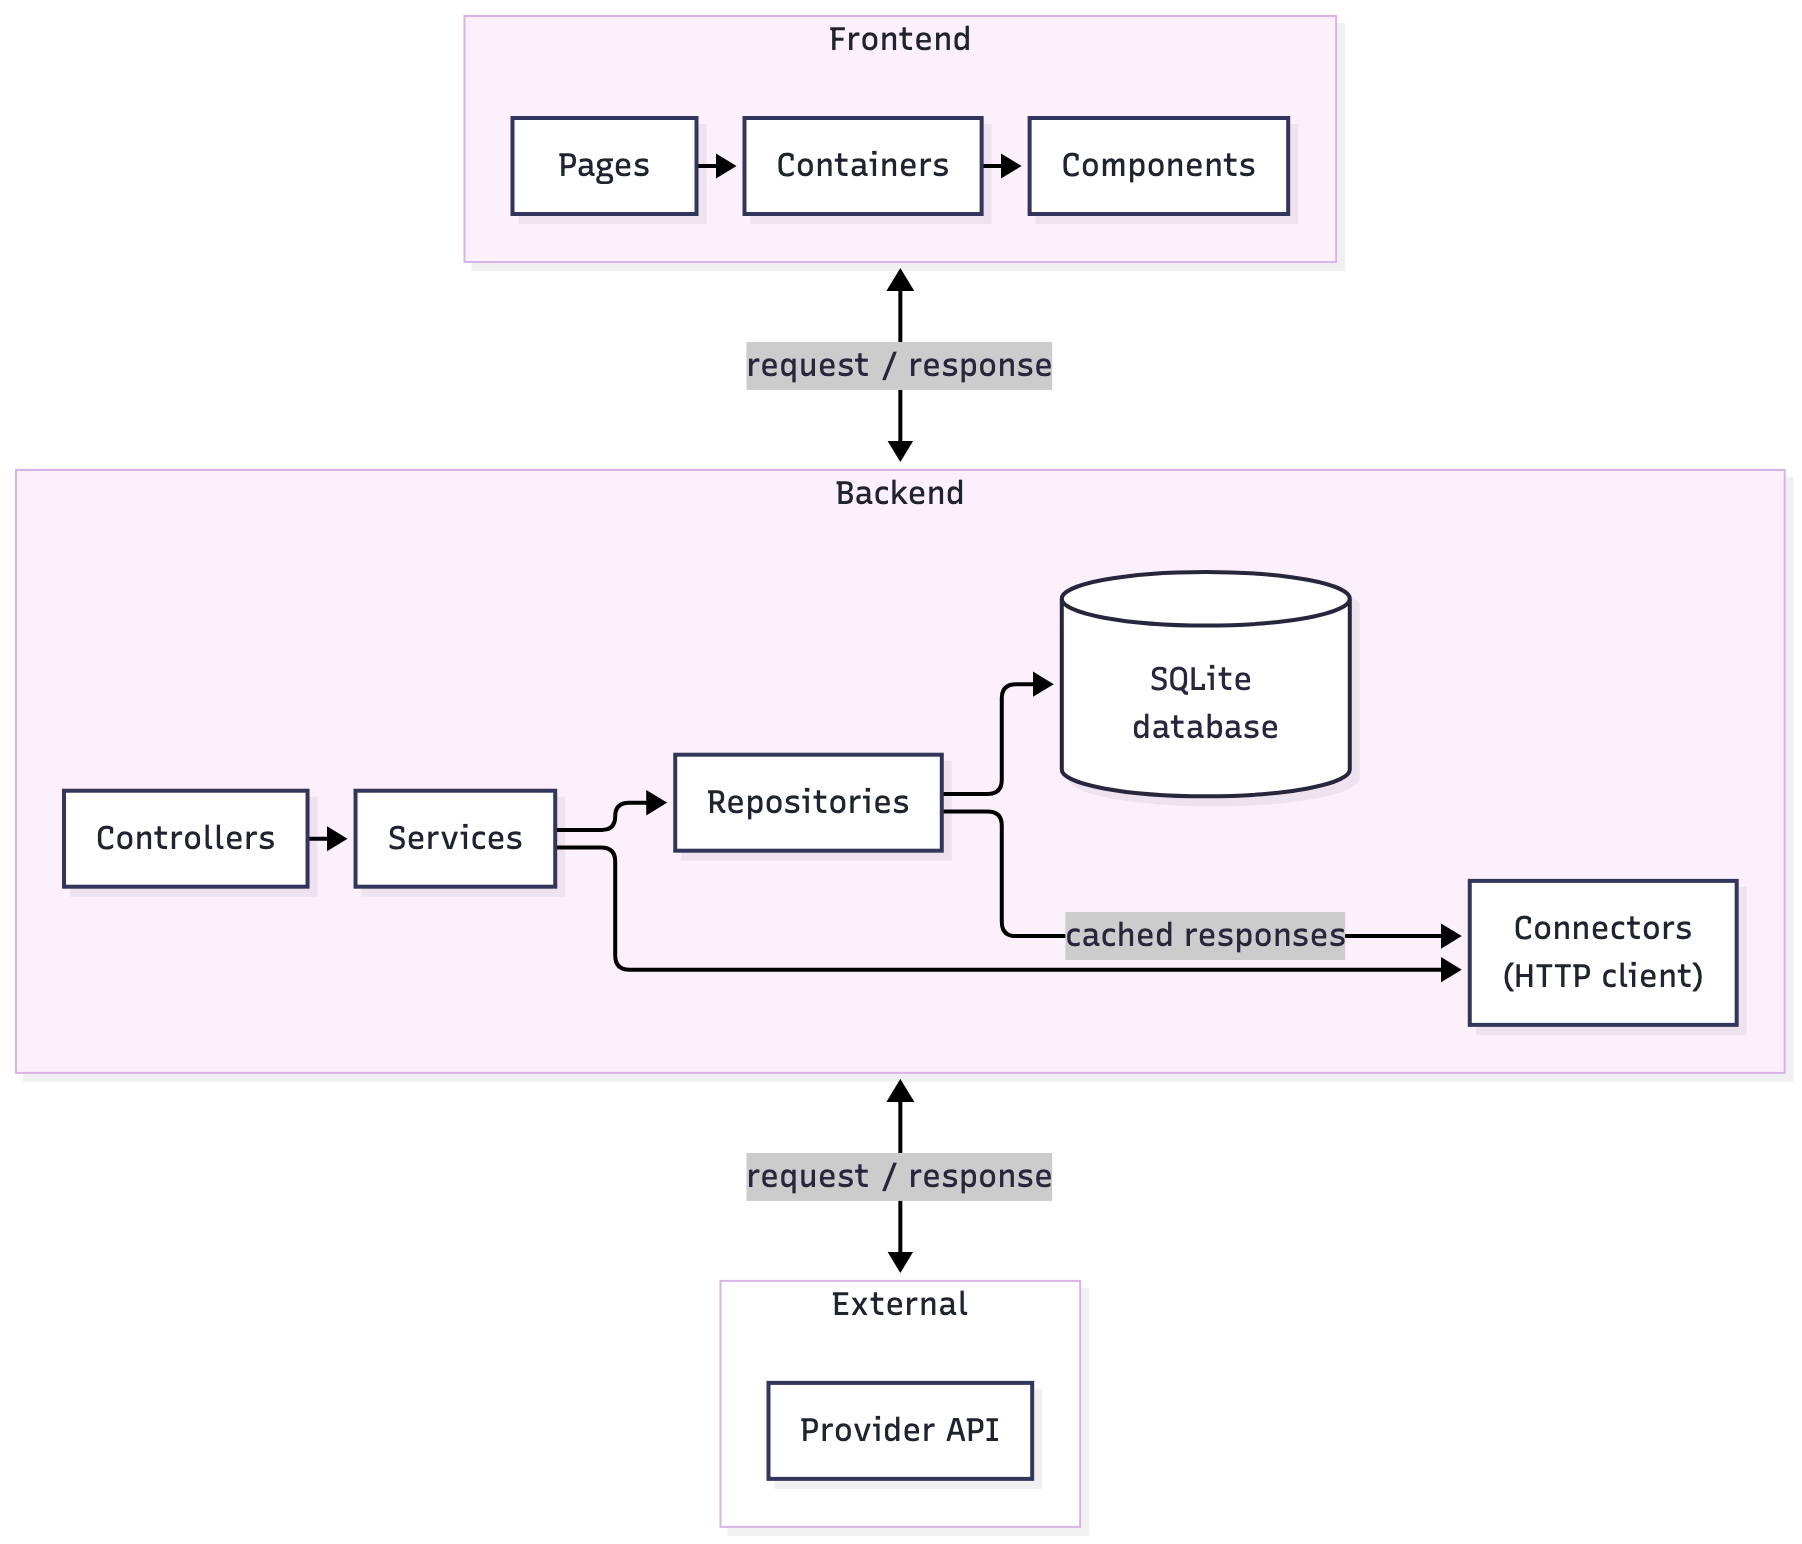
\includegraphics[scale=.2]{include/fig-arch-mvc-diagram}

    \caption{MVC architecture overview}
    \label{fig:mvc-pattern}
\end{figure}

The system design follows the Model-View-Controller (MVC) architectural pattern.
Figure~\ref{fig:mvc-pattern} outlines the architectural structure.


The user interface (UI) consists of a web page (frontend). 
It connects to the backend service, which encapsulates the business logic, and exposes the functionality via an Application Programming Interface (API).

Both system modules (frontend and backend) are written in \textsf{JavaScript}: the frontend is built with \textsf{React}, the backend targets \textsf{Node.js}.
The frontend does not implement any meaningful reusable business logic, instead it forwards the requests to the backend and displays the results.
The backend communicates with the external data sources to gather information, and performs citation analysis.

\subsection{Backend} \label{sec:backend-layers}

The backend is structured in layers of data flow separation.
The layers and components are introduced below. 

\subsubsection{Services}

Services is the only component containing the business logic to coordinate the collection and analysis of data.

Services are classes corresponding to entity domains, exposing methods that provide the functionality expected of each entity.
They never see the request or the response objects.
Instead, they receive transformed and sanitized arguments, and return data structures corresponding to their own internal model.
This separation keeps the business logic independent of the transport protocol: the same service can be invoked by a controller, injected into another service, or unit tested.
There is one service for each subject:
\begin{enumerate}
\item
\textsf{AuthorService} for author profiles, 
\item
\textsf{PublicationService} for papers and citations, 
\item
\textsf{ClassificationService} for the classification algorithm, 
\item
\textsf{CitationGraphService} for operations on the citation graph as a whole, 
\item
\textsf{JobService} for the background jobs, and 
\item
\textsf{MetricsService} for the count aggregation.
\end{enumerate}

Dependencies are injected into each service to provide the underlying functionality needed to produce the results.
For instance, the \textsf{MetricsService} orchestrates the flow to produce the citation collection described in Section~\ref{sec:processing-pipeline}: it requests the papers of the selected author by calling the \textsf{AuthorService}, the citations of each paper through the \textsf{PublicationService}, and the classification of each citation through the \textsf{ClassificationService}, to finally hand the assembled graph to the \textsf{CitationGraphService} to be stored.

\subsubsection{Connectors}

Connectors handle the fetching and processing of data from external sources.

Connectors are also classes, one per provider, implementing the communication with external data sources; no other component is allowed to contact a provider directly, instead all requests for external data go through the connectors.
Every connector implements the same interface (\textsf{ProviderConnector}) with the operations described in Section~\ref{sec:providers}, so the rest of the system treats all sources in the same manner.

A connector transforms the responses into the internal model, that is used by the rest of the system.
All provider specifics are isolated inside the respective connector: the endpoint structure, the request and response models, pagination, authentication etc.
For instance, the \textsf{OpenAlex} connector paginates with 200 records per page, and the \textsf{Google Scholar} connector is limited to 20 records per page; both return the same data structure, regardless of how they gather the results.

\subsubsection{Controllers}

Controllers receive user requests and pass them to services.

Controllers are classes with one method for each API endpoint that the backend exposes.
They contain minimal business logic, limited to the endpoint structure, as a function of the interface that the service provides.
Their responsibility is to validate the incoming parameters, transform the requests into the internal model, call the respective service, transform the service result into a response.
For instance, a search request without a query parameter is rejected with a status code \textsf{400}, not having reached a service.
Controllers are separated by the use cases.
There is \textsf{SearchController} for the author search, \textsf{AuthorController} for the author details, papers and stored metrics, \textsf{JobController} for submitting jobs and polling their status, and \textsf{StatusController} for the provider quotas and system resources.

\subsubsection{Repositories}

Repositories read from and write to the database tables.

Repositories, too, are classes with methods, implementing the functionality that depends on connection to the database; no other component is allowed to make database queries directly, instead all requests for data go through the methods exposed by the repositories.
There is one repository for each table: \textsf{publications}, \textsf{authors}, \textsf{contributions}, \textsf{citations}, \textsf{cache} and \textsf{jobs}.

Repositories implement only the SQL operations that the application needs, not every possible operation on every table.
They expose arbitrary methods, for instance to save items or to find records by different criteria.

Instead of writing the queries directly in SQL and sending them through the database driver, the repositories use an object-relational mapping (ORM) library (\textsf{Drizzle}\footnote{\url{https://orm.drizzle.team}}).
The schema of tables and columns is declared in code, as described in Section~\ref{sec:storage-caching}, and the queries are expressed as code as well, to allow this layer of the system to be statically analyzed and unit tested, just like the rest of the project.

As the repositories are isolated per entity, only the relevant repositories are injected into the respective services.
For instance, the citation graph service (\textsf{CitationGraphService}) needs to read and update the tables \textsf{publications}, \textsf{authors}, \textsf{contributions} and \textsf{citations} to save a collected graph and load it back, so the four respective repositories (\textsf{PublicationRepository}, \textsf{AuthorRepository}, \textsf{ContributionRepository}, \textsf{CitationRepository}) must be provided in the constructor.

\subsection{Frontend} \label{sec:frontend-layers}

The frontend serves as a presentation layer and interface controller, and follows a data flow similar to the backend.
The building blocks of the UI are \emph{components}, \emph{containers}, and \emph{pages}.
Figure~\ref{fig:frontend-components} shows how the frontend is composed and how it connects to the backend. 

\begin{figure}[tb]
    \centering
    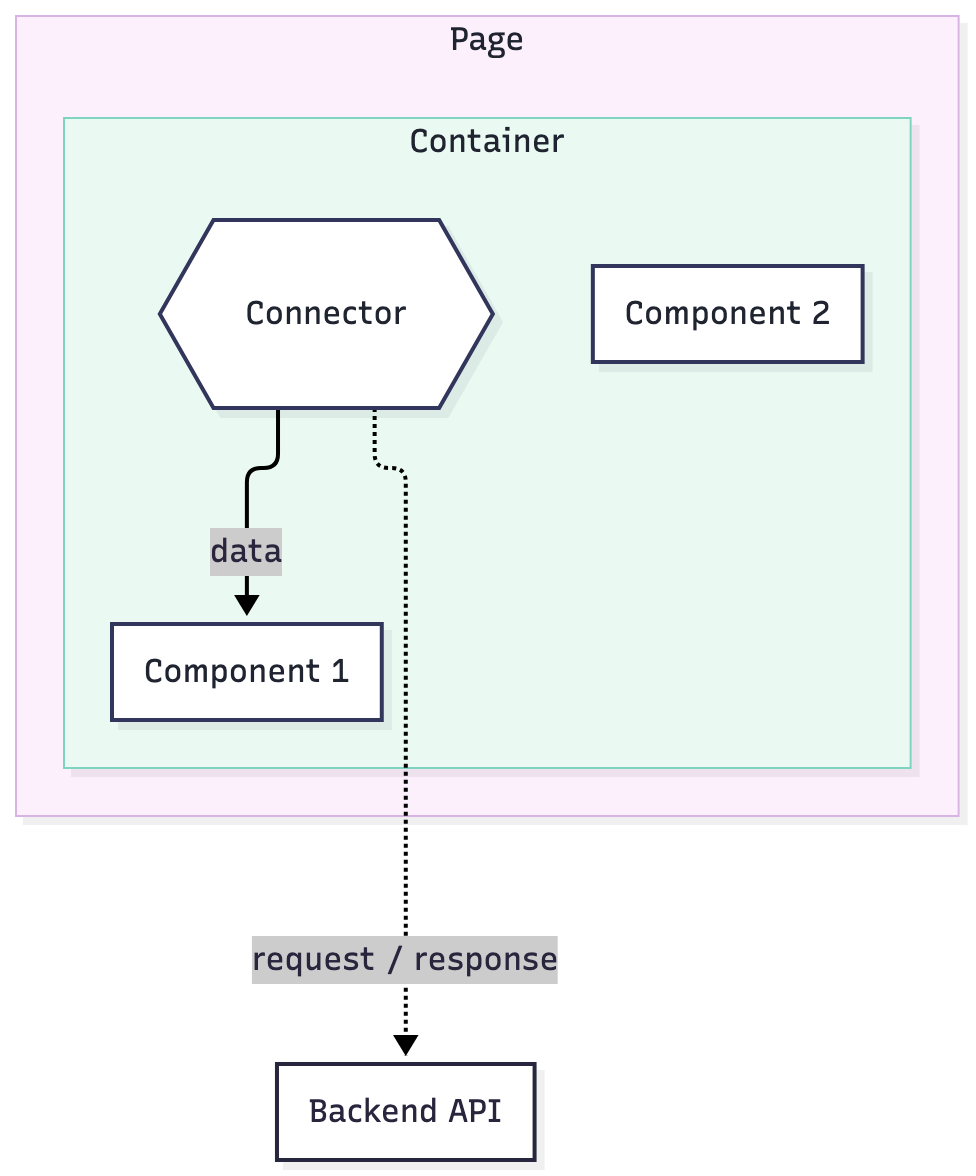
\includegraphics[scale=.2]{include/fig-frontend-component-diagram}

    \caption{Frontend building blocks: pages, containers and components}
    \label{fig:frontend-components}
\end{figure}


\subsubsection{Components}

Components are the reusable atomic widgets that define how a piece of data should look and behave.
They are not responsible for retrieving the data, only for rendering and styling it.
For example, a loading indicator or an error message are components, and can be used on different occasions by different containers.

\subsubsection{Containers}

Containers are meaningful groups of related components.
They manage and request data, implement all the presentation logic around orchestration of the components.
They are responsible for calling the API, showing the loading or error state, as well as wiring together the components and supplying the data to them.

\subsubsection{Pages}

Pages are the largest units of the frontend, each page usually corresponds to a unique path of the address in the browser.
The application currently consists of two pages: author search (\texttt{/authors}) and author details (\texttt{/author/:provider/:authorId}).
Each page is built with one or more containers.

The backend performs the retrieval as an asynchronous background job, to provide progress while collecting data, which can potentially take time, especially for authors with many publications and sources with low throughput.
The frontend polls and displays the progress of these jobs in the UI.

The following sections describe the provider choices, data model and processing steps in more detail.

%\enote{done (mermaid is my tool)} \snote{Fine, but also put the sources in the repo. } \enote{done (previously they were all in the system-design.md, extracted also into docs/fiagrams; build by `make diagrams`)}

\section{Providers and limitations} \label{sec:providers}

Citation sources were analyzed in Section~\ref{sec:data-sources} by the supported data properties and the provided access methods (see also Figure~\ref{fig:providers-overview}). Among these, three data providers were supported in our system implementation, namely: 
\begin{enumerate}
\item
\textsf{OpenAlex}\footnote{\url{https://openalex.org}}, 
\item
\textsf{Semantic Scholar}\footnote{\url{https://www.semanticscholar.org}}, and
\item
\textsf{Google Scholar}\footnote{\url{https://scholar.google.com}} (via \textsf{SerpApi}\footnote{\url{https://serpapi.com}}).
\end{enumerate}
\textsf{OpenAlex} and \textsf{Semantic Scholar} are the most naturally fitting open sources.
Their responses to requests for citations also include author lists, needed by the classification algorithm.
\textsf{Google Scholar}, as the one with the widest coverage, was also considered, despite all the limitations around using it.
The remaining sources were not considered:

\begin{description}
    \item \textsf{CrossRef}\footnote{\url{https://www.crossref.org}} does not list the citing papers.
    \item \textsf{OpenCitations}\footnote{\url{https://opencitations.net}} does not support search by author name (only by identifier).
    \item \textsf{DBLP}\footnote{\url{https://dblp.org}} is limited to computer science and does not provide citations.
    \item \textsf{Scopus}\footnote{\url{https://www.scopus.com}} requires a paid institutional subscription.
\end{description}


%Figure~\ref{fig:providers-overview} shows the provider connectors.

\begin{figure}[tb]
    \centering
    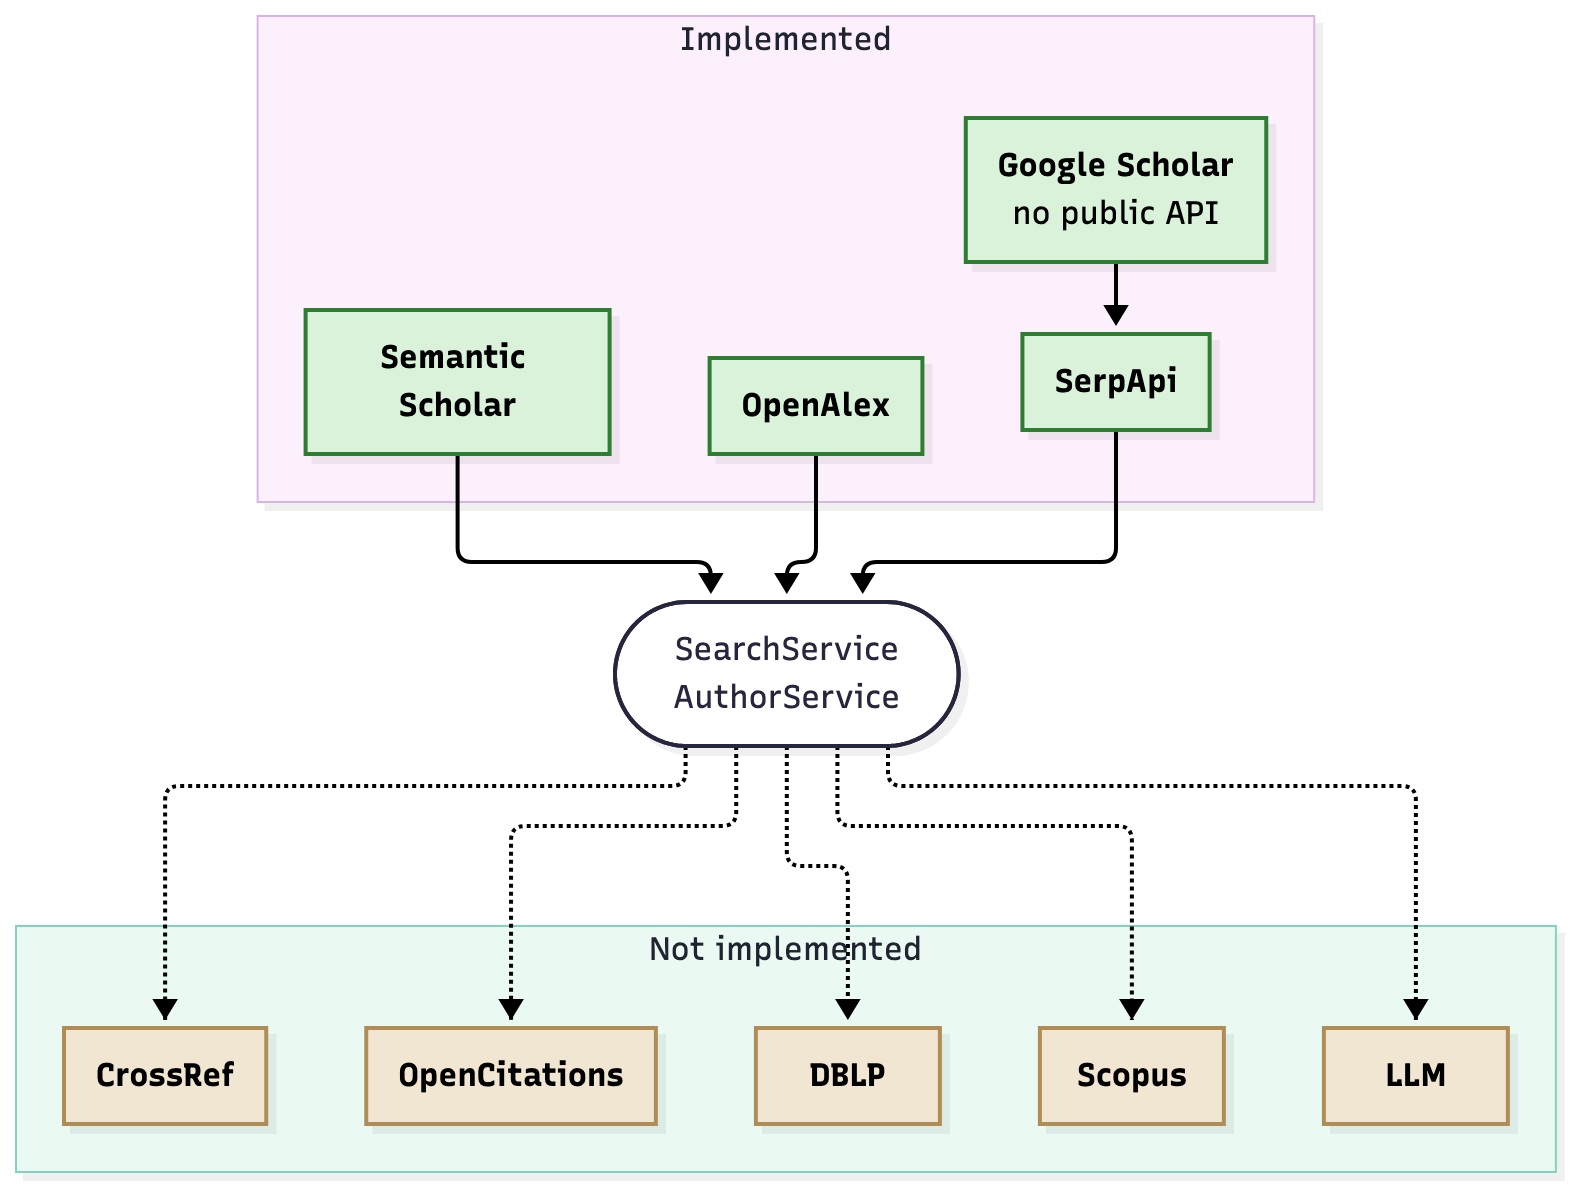
\includegraphics[scale=.2]{include/fig-providers-diagram}
    \caption{Providers and their respective connectors}
    \label{fig:providers-overview}
\end{figure}

In the backend, each data source is reached through its own \emph{connector}, to isolate the differences in access and the structure of data it returns.
Every connector implements the interface \textsf{ProviderConnector}, defining the operations:

\begin{description}
    \item \textsf{searchAuthors} to find an author,
    \item \textsf{getAuthorPublications} to list author papers,
    \item \textsf{getCitations} to list paper citations.
\end{description}

The remaining system builds on top of these operations, treating all sources in the same manner.
As the connectors are interchangeable, a source may be added or replaced without changing the remaining processing pipeline.
At the same time forensic bug investigation for each source remains within its own connector, making it easy to locate problems and test behavior.

Each provider imposes a concurrent request throttling.
The implementation uses asynchronous queues to stay within the rate limits.

None of the sources considered for this project shares author identifiers fully compatible with another.
The profiles are kept separate and shown side by side, as described in Section~\ref{sec:system-overview}.

The largest source (\textsf{Google Scholar}), even when accessed via a paid proxy (\textsf{SerpApi}), is the most restrictive in practice.
Collecting the citations of an author with $n$ publications requires at least $n$ requests, growing the cost proportionally to the volume of data retrieved.
The free sources (i.e., \textsf{OpenAlex} and \textsf{Semantic Scholar}) are used by default in the system.

\section{Data} \label{sec:data}

The conceptual model described in Section~\ref{sec:data-model} translates to four domain-specific tables: \textsf{authors}, \textsf{publications}, \textsf{contributions}, and \textsf{citations}.
There is also a table to save the asynchronous jobs state (\textsf{jobs}), and a table for cached responses (\textsf{cache}), described in Section~\ref{sec:storage-caching}. 
Figure~\ref{fig:database-er} shows the database tables and the relationships between them.

\begin{figure}[tb]
    \centering
    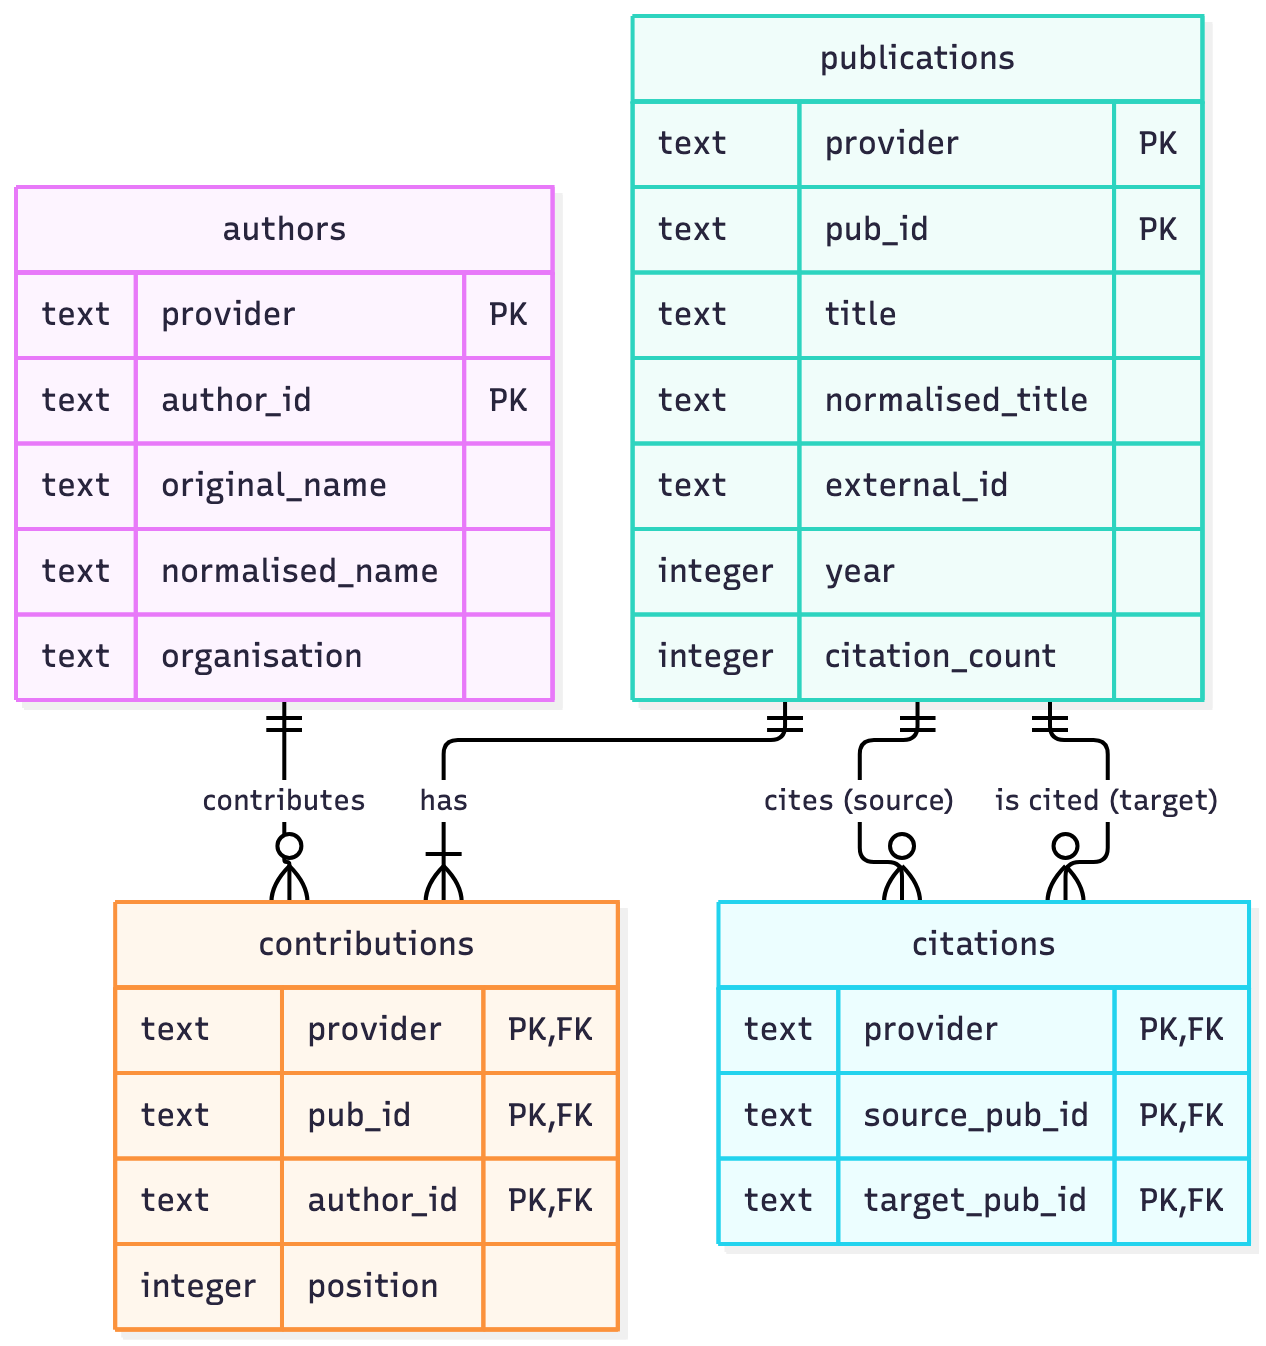
\includegraphics[scale=.2]{include/fig-database-er-diagram}
    \hspace{2em}
    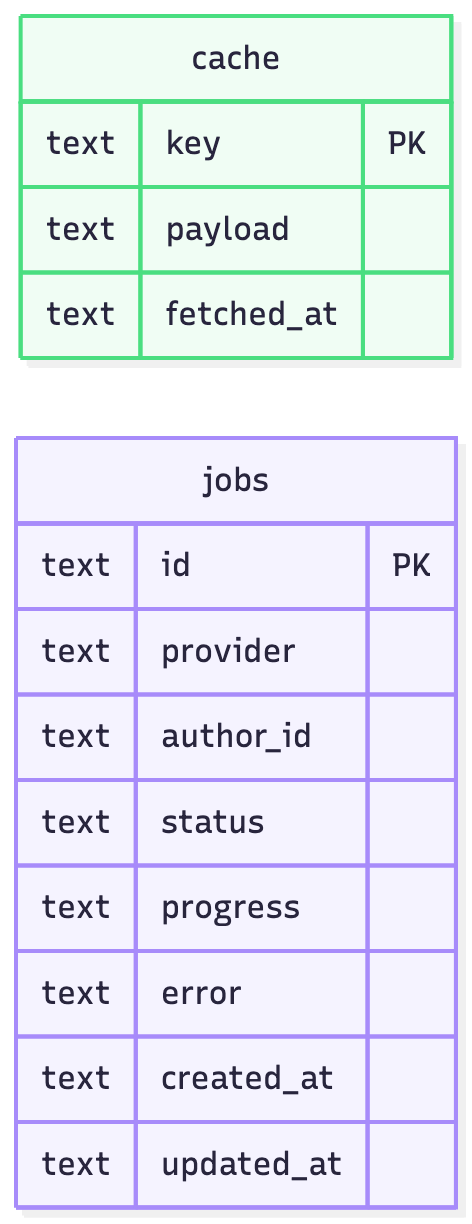
\includegraphics[scale=.2]{include/fig-database-aux-er-diagram}
    \caption{Database tables}
    \label{fig:database-er}
\end{figure}

In the conceptual model, a publication is identified by its title, year and authors, and an author by name.
The implementation uses the identifiers assigned by each provider: \textsf{pubId} and \textsf{authorId}.
Names and titles can be ambiguous, and spelling differences do not necessarily mean that two records refer to different entities.
All primary keys are composite and include the provider identifier, to keep the data separate by provider.

A \textsf{publication} record contains the title, year, citation count reported by the provider, and an external identifier, for instance a DOI, if available.
An \textsf{author} record consists of the name and the affiliation, if available.
A \textsf{contribution} record connects an \textsf{author} to a \textsf{publication}; it includes the position of each one of the list of paper authors.
A \textsf{citation} record connects the \textsf{citing publication} (source) to the \textsf{cited publication} (target).

Normalized author names and paper titles are stored in the respective entity tables, alongside the original names and titles.
The normalization consists of simple string manipulations, such as conversion to lower case, removal of diacritics, and replacement of repeated whitespace.
For example, \emph{Skiadópoulos} and \emph{skiadopoulos} produce the same normalized value.

\textsf{OpenAlex} and \textsf{Semantic Scholar} typically return authors and publications with their own internal identifiers.
Their connectors filter the list of contributions to remove ones without an author identifier.
The \textsf{Semantic Scholar} connector also discards citing papers without a paper identifier.

\textsf{Google Scholar} does not guarantee to return identifiers for the authors of citing papers, often it returns names as strings, which are inherently unreliable for uniquely identifying anything.
When an identifier is missing, the respective connector uses the normalized name, but this remains a known issue, leading to self-citations being potentially under-represented in the \textsf{Google Scholar} results.

\section{Storage and caching} \label{sec:storage-caching}

\textsf{SQLite} was used in the system for the simplicity of its setup.
It does not require a separate server, instead the database file (it is a single file) is opened directly by the backend server process, all updates and changes are stored in it, and it is closed when the server shuts down and closes the database connection.

The database schema is only defined in the code, in a single file describing every table, index, and column relationship.
When the schema changes, the ORM compares it with the previous version and generates code representing the migration, as part of the backend build pipeline.
A migration is a file with SQL statements needed to change the current database schema to the new schema.
Migrations are kept in the codebase too, and are checked into the version control system.
Every time the backend starts up and opens the database, it applies the migrations that have not been applied yet.
Using this approach, the database schema always starts from the initial empty state, it then grows, and eventually evolves into the final version of the schema needed by the application.

The system largely depends on externally sourced data, subject to the provider limitations and the latency of network access.
Publications, authors, contributions and citations are treated as immutable in nature.
These details, when retrieved and linked together, form a graph of nodes and relationships, coined as \emph{citation graph}. 

The citation graph is a two-dimensional representation of the conceptual domain model.
In this graph, \emph{publications} and \emph{authors} are the nodes of this graph, \emph{contributions} and \emph{citations} are the two types of directed edges.

The graph can be pivoted to center around any author, producing three levels of layering.

\begin{description}
    \item [Selected author] is connected to their own papers (as \emph{contributions}).
    \item [Citing papers] are connected to the selected author papers (as \emph{citations}).
    \item [Citation authors] are connected to each citing paper (as \emph{contributions}).
\end{description}

The citation graph is decomposed and stored as separate entities in the tables
\textsf{publications}, \textsf{authors}, \textsf{contributions} and \textsf{citations} (Figure~\ref{fig:database-er}), as described in Section~\ref{sec:data}. 

The citation graph described in Section~\ref{sec:user-interface} represents the citations graph visually.

After collecting the data, the backend saves the publications, authors and their relationships, from which the graph can be reconstructed without network requests to external providers.
Classification labels depend on the choice of author (the same citation can be \textsf{direct} for one author and a \textsf{co-author self-citation} for another) and are calculated at runtime, when the graph is loaded.
Figure~\ref{fig:classification-example} shows the classification of the same citation for different authors, involved in either or both of the papers.

As an example, let us consider the publications discussed in Chapter~\ref{c1:intro}.
Publication~\cite{Kalnis2007} by Kalnis, Ghinita, Mouratidis and Papadias cites publication~\cite{Ghinita2007} by Ghinita, Kalnis and Skiadopoulos.


The citation classification changes depending on who is the author under analysis.
For \emph{Kalnis} or \emph{Ghinita}, as authors of both papers, the citation classification is \textsf{direct self-citation}.
If the author under analysis is \emph{Skiadopoulos}, who only appears on the cited publication, the classification cannot be \textsf{direct self-citation}.
As other authors of the cited paper also appear on the citing paper, the classification is then \textsf{co-author self-citation} for Skiadopoulos.

\begin{figure}[tb]
    \centering
    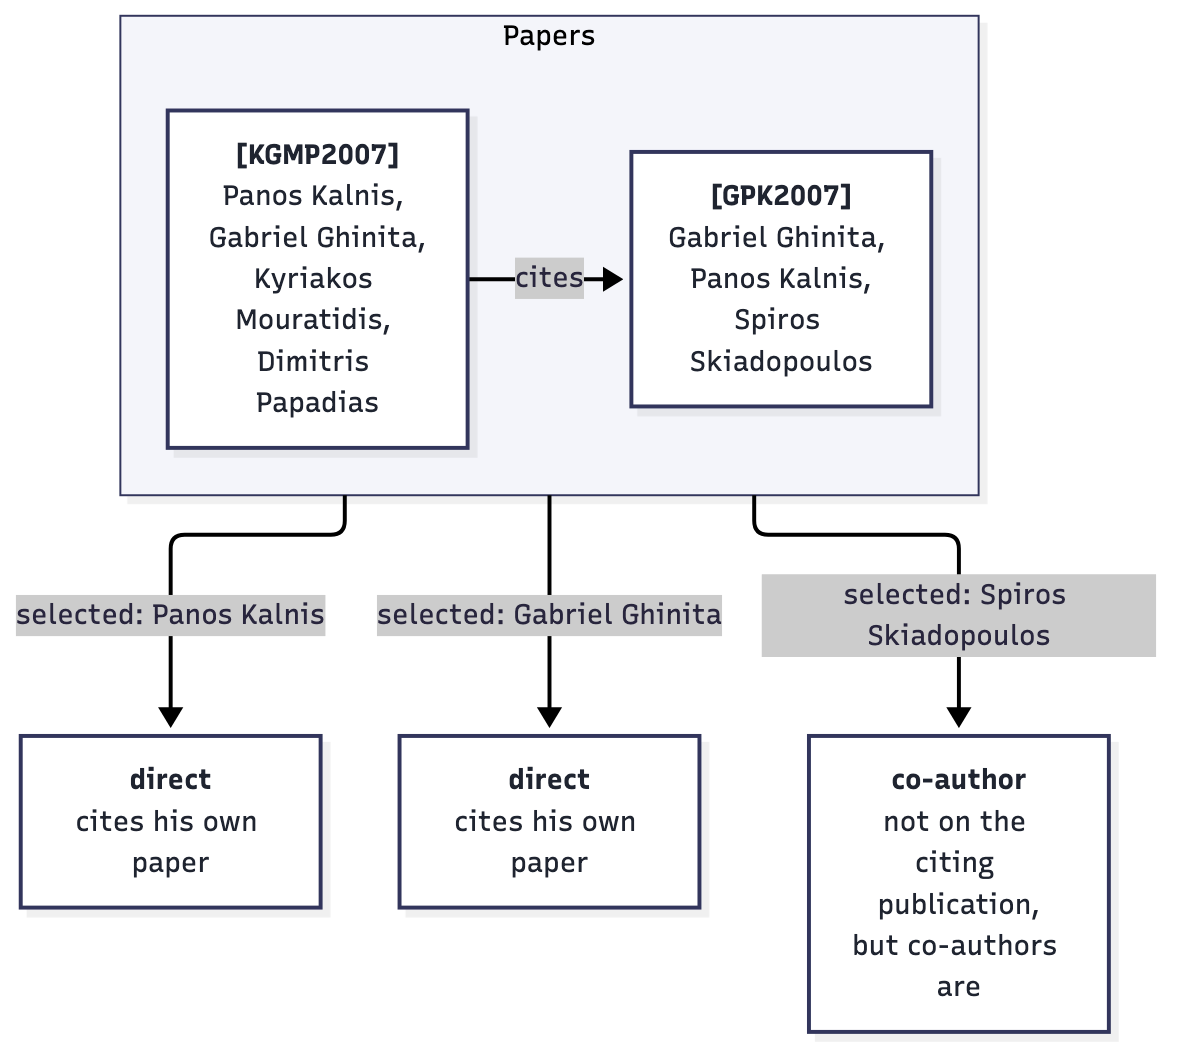
\includegraphics[scale=.2]{include/fig-classification-example-diagram}
    \caption{Classification of the same citation for each selected author}
    \label{fig:classification-example}
\end{figure}

Figure~\ref{fig:cache-flowchart-diagram} illustrates the data flow inside the cache mechanism.
All provider connectors use the same HTTP client implementation, with caching handled internally.
Before sending a request, the client looks for a stored response using the request URL as the key.
The cache key enforces the order of the query parameters alphabetically, to provide a stable key, regardless of the parameter order in the original request URL.
For instance, \texttt{https://example.com?p1=v1\&p2=v2} and \texttt{https://example.com?p2=v2\&p1=v1} produce the same key.
Each cached record includes the date it was received, used to calculate when the record satisfies the time-to-live timeframe.

\begin{figure}[tb]
    \centering
    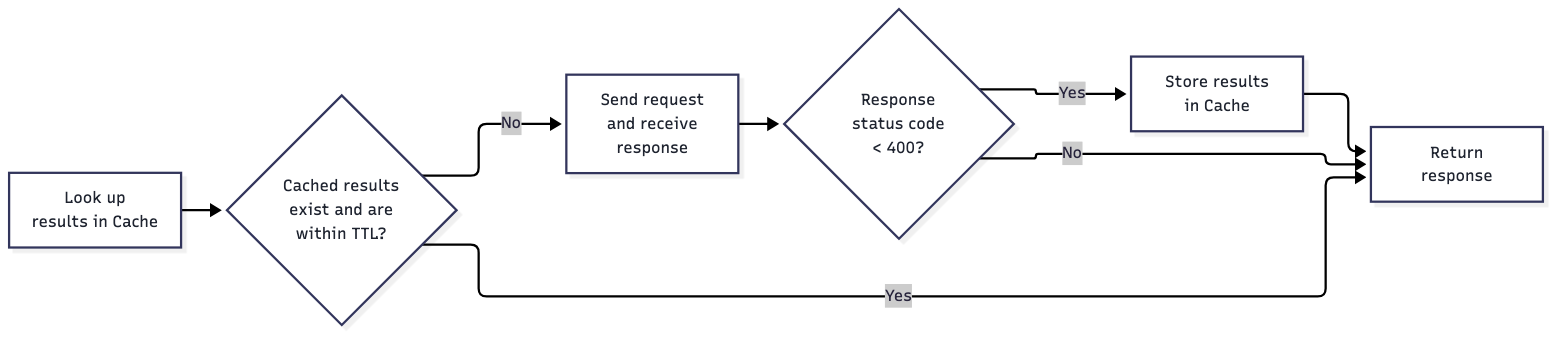
\includegraphics[scale=.2]{include/fig-cache-flowchart-diagram}
    \caption{Cache request data flow}
    \label{fig:cache-flowchart-diagram}
\end{figure}

If the record is found, and it has not expired, the response contained within is returned; otherwise, the request is sent to the provider.
Successful responses are stored as text under the same key and with the current date.

Expired cache records are replaced when requested again, but there is no periodic deletion of old entries, and there is no limit on the cache size.
The database can grow forever, which is a limitation of a shared installation, that would need a retention policy and clean up procedures.

\section{Processing pipeline} \label{sec:processing-pipeline}
Once the user has selected the author, the UI automatically checks if a citation graph for this author exists in the system for the currently selected provider, using the date of the last completed job for this author and provider, which the backend returns with the author details.
If the citation graph exists, it is returned as a raw dataset in JSON format, and that date is shown as the time of the last update.
The UI renders results, including an option to update the results, bypassing the previously stored graph and cache.
If the citation graph does not exist, or the user has requested to update the results, the backend receives a request to fetch the full graph.

Having received a request to fetch the full graph from a provider, the backend creates a new job (as an in-memory object) and stores it in the database.
The job is initially placed in the \textsf{running} state, which is the only non-final state.
The backend immediately responds with the job object, including the identifier.
With the identifier at hand, the client starts to poll the job status, until it reaches one of the final states, namely, \textsf{done}, \textsf{error}, or \textsf{interrupted}.

Meanwhile, in the background, the backend orchestrates the flow to build the citation graph.
Figure~\ref{fig:classification-flowchart-diagram} illustrates the data flow of constructing the full graph from an author identifier.
The successful path is as follows:

\begin{itemize}
    \item The \textsf{Metrics service}, which orchestrates the flow, hands it over to the \textsf{Author service}.
    \item The \textsf{Author service} requests the list of papers for the selected author identifier, and paginates to reach the end of the response list.
    \item Having reached the end of the list, the \textsf{Author service} calls the \textsf{Publication service} to fetch the citations, for each of the gathered publications
    \item The \textsf{Publication service} requests the list of citations, and extracts the authors from each item of the list.
    In practice, the requests for all publications are queued in bulk, at the same time, and the per-provider request queue dispatches them sequentially, limiting concurrent requests to the number of requests per second that the provider allows.
    \item Having gathered details of each of the citing publications, the control returns to the \textsf{Metrics service} to aggregate final results.
    \item The \textsf{Classification service} applies the classification algorithm to each of the citing publications against the author under analysis.
    \item The \textsf{Metrics service} collates the results into a single nested structure, stores it in the database, and changes the job status to \textsf{done}.
\end{itemize}

If the citations of a publication cannot be retrieved, for instance due to a network error, this publication is skipped.
The job will still complete, and the result will mention how many responses were successful and how many failed.

Once the job has been updated with the final result, the next time the client requests the job, it will receive the result and will be able to fetch it and render in the UI.

\begin{figure}[tb]
    \centering
    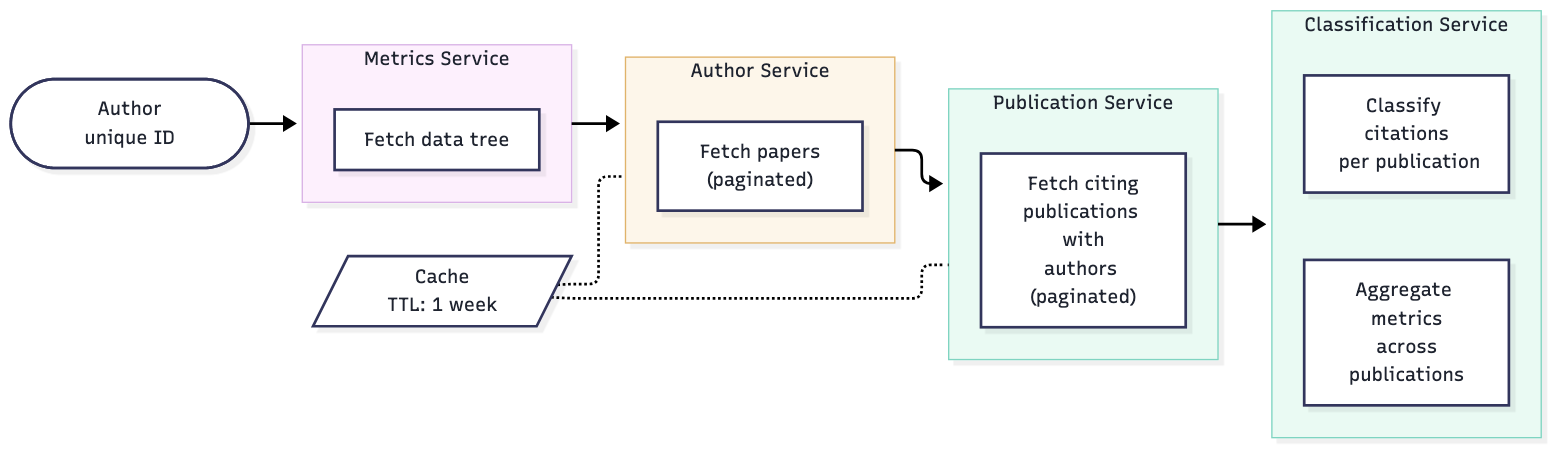
\includegraphics[scale=.2]{include/fig-classification-flowchart-diagram}
    \caption{Citation graph construction data flow}
    \label{fig:classification-flowchart-diagram}
\end{figure}

\section{User interface} \label{sec:user-interface}

The software application responsible for interaction with the user, user interface (UI), consists of a single-page web application.
User interface addresses the use cases described in Section~\ref{sec:system-overview}: finding an author, and getting citation metrics for a selected author.
The application consists of a few individual components described below: \textsf{Search form}, \textsf{Search results}, \textsf{Author details}, \textsf{Status}.

\subsection{Search form} \label{sec:ui-search-form}

Figure~\ref{fig:ui-search-form} shows the initially empty search page, where the user enters a name to start the flow of selecting an author.
Currently, there is no way to disable or enable some of the providers, this setting is controlled by the backend.

The page supports deep-linking to the search form with the name prefilled, when the URL specifies the parameter \texttt{q=query}, for instance \texttt{http://localhost:3000/authors?q=skiadopoulos}.

\begin{figure}[tb]
    \centering
    
\includegraphics[scale=.4]{include/ui/search-form-1}

\snote{crop the white part. You do not need it!}
    \caption{Author search form}
    \label{fig:ui-search-form}
\end{figure}

\subsection{Search results} \label{sec:ui-results}

Figure~\ref{fig:ui-search-results} shows the search results page, displayed after the search form has been submitted, and the response has been returned.

Searching by name can return multiple results, matching the name, for each of the supported providers; the figure shows the list of results returned for \texttt{skiadopoulos}.

\begin{figure}[p]
%\begin{figure}[tb]
\snote{An idea when you have to many figures is to use [p] that puts them in a single page. Here it looks good this way!}
\enote{I actually tried with [h] - here, and it looked maximum satisfactory, as it was right where the text spoke about it. but I assume it isn't what the reports usually do.}

    \centering
    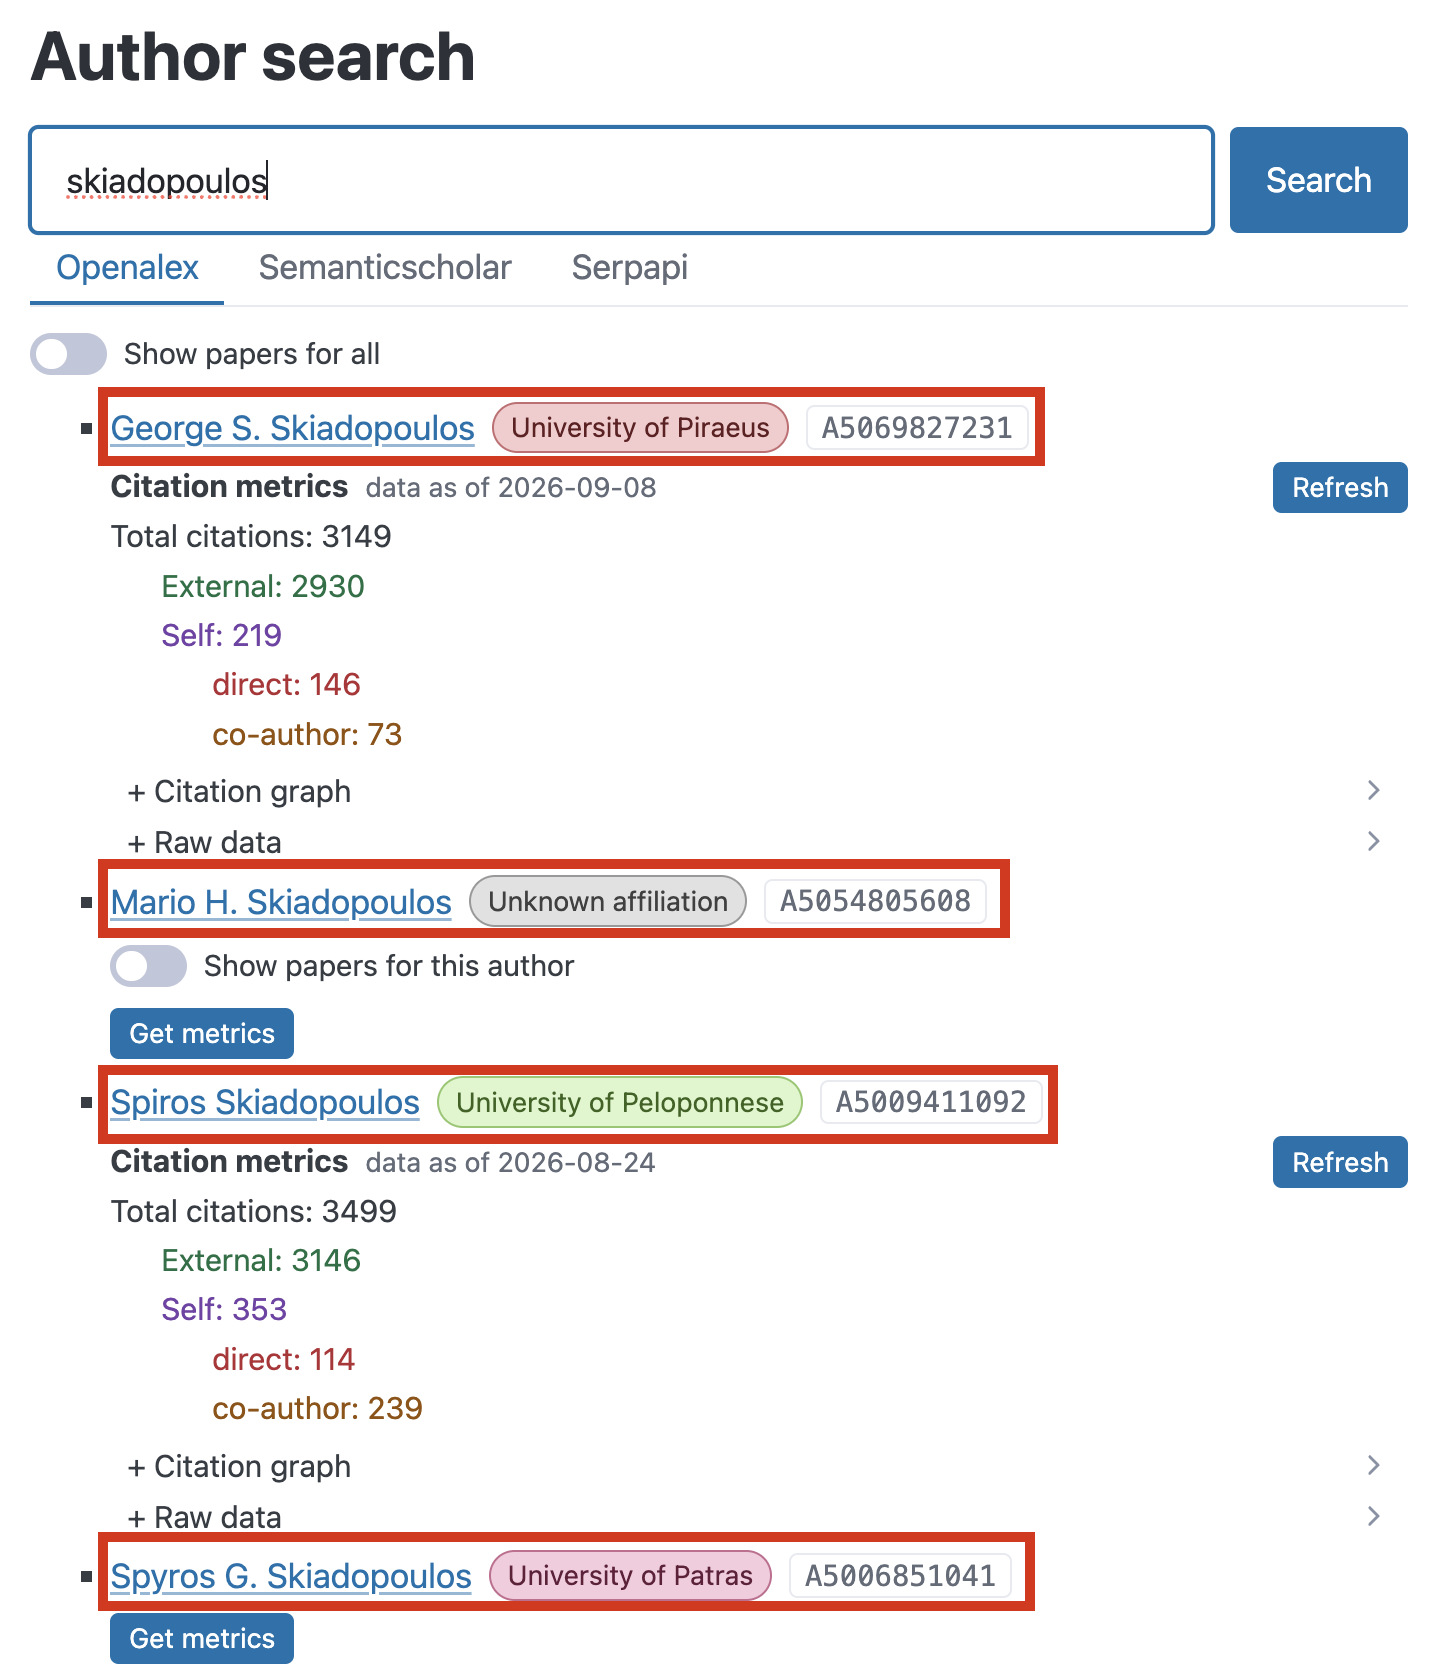
\includegraphics[scale=.4]{include/ui/search-res-1}
    \caption{Authors returned by one of the providers}
    \label{fig:ui-search-results}

    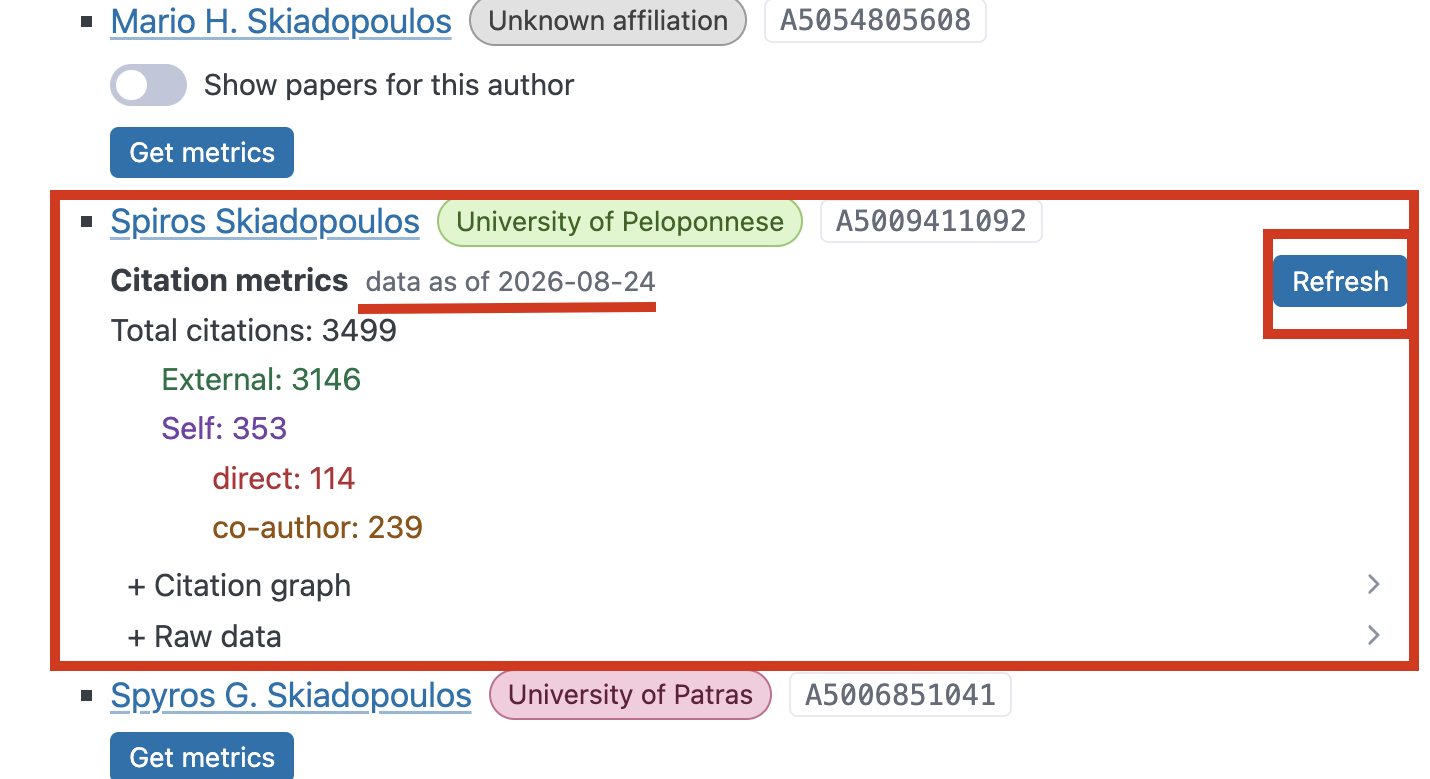
\includegraphics[scale=.4]{include/ui/search-res-2}
    \caption{Stored citation metrics, update date and refresh button}
    \label{fig:ui-search-controls}

\end{figure}

Each author name on the result list is accompanied by an affiliation, when available, and the identifier assigned by the selected provider.
The name is a link to the author detail page, described in Section~\ref{sec:ui-details}.

Figure~\ref{fig:ui-search-controls} shows the stored metrics, the update date and the refresh button of a profile.
The profiles, where results have not been collected previously, include a \emph{Get metrics} button \snote{Ideally, buttons should look as it is in the figure, but do not try hard to do it. Only if it does not take time and energy! An inline includegraphics might to the trick.}, to request the citation counts.
For profiles, where citation metrics have previously been requested, and the citation graphs are found in the database, the UI shows the metrics and the date of the last update.
For these profiles there is a \emph{Refresh} button to request the data, ignoring the stored graph and cached responses.

%\begin{figure}[tb]
%    \centering
%    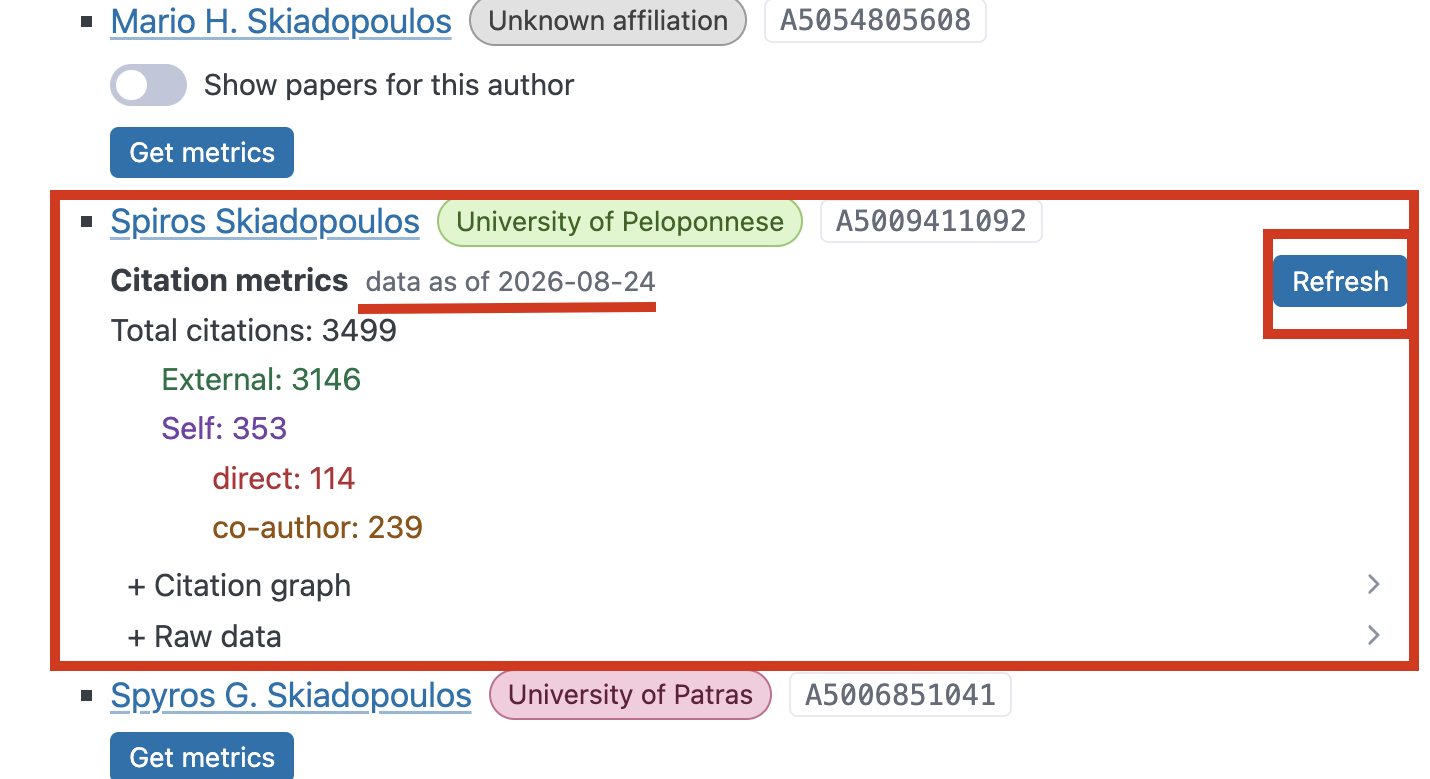
\includegraphics[scale=.4]{include/ui/search-res-2}
%    \caption{Stored citation metrics, update date and refresh button}
%    \label{fig:ui-search-controls}
%\end{figure}

Figure~\ref{fig:ui-provider-tabs} highlights the selected provider.
The provider tabs keep results isolated per source, following the decision described in Section~\ref{sec:providers}.

\begin{figure}[tb]
    \centering
    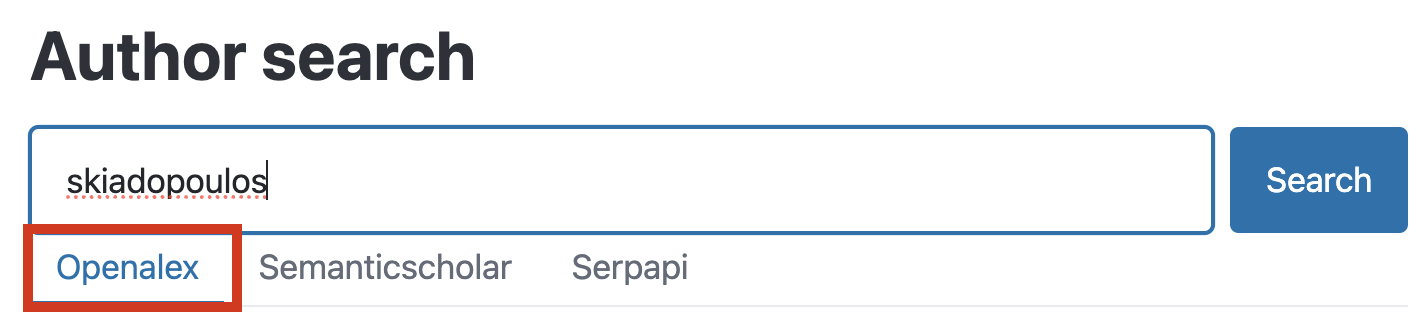
\includegraphics[scale=.4]{include/ui/search-res-4}
    \caption{Provider tabs in the search results}
    \label{fig:ui-provider-tabs}
\end{figure}

If search fails for a provider, its tab will display an error, not affecting the results of the other providers.

Figure~\ref{fig:ui-show-papers} shows the \emph{Show papers for all} switch, which applies to all the authors in the selected tab.
To help deterministically select the correct author, among ones with similar names and affiliations, the UI provides an option to display their publications.
A familiar title could be easier to recognize, especially if the author has changed affiliation, or shows no affiliation in the UI.

\begin{figure}[tb]
    \centering
    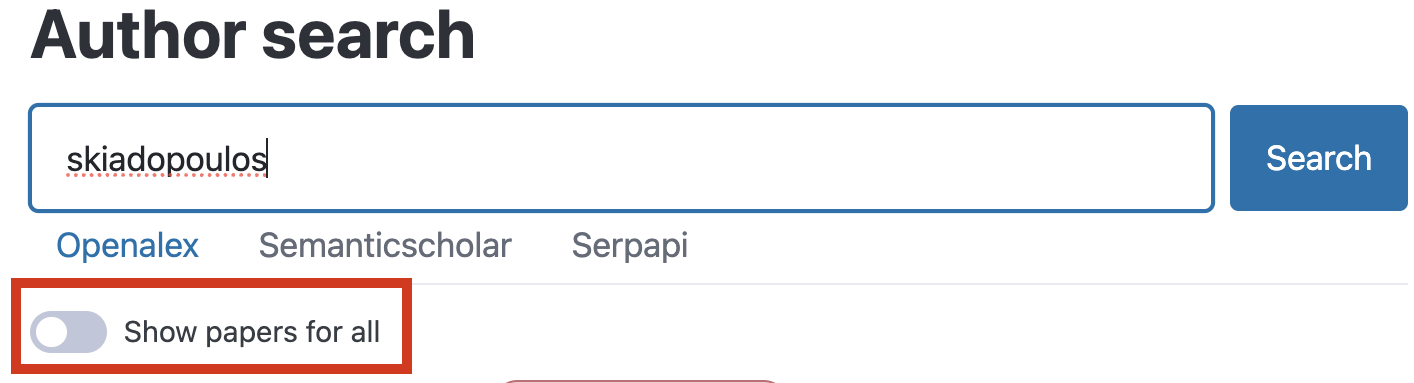
\includegraphics[scale=.4]{include/ui/search-res-5}
    \caption{Showing papers for all authors}
    \label{fig:ui-show-papers}
\end{figure}

Figure~\ref{fig:ui-unknown-affiliation} shows a profile without an affiliation, displayed as \emph{Unknown affiliation}: only such profiles include a switch to show the papers of the individual author.
This is helpful to avoid waiting for other authors on the list, and consuming the provider quotas.

\begin{figure}[tb]
    \centering
    
\includegraphics[scale=.4]{include/ui/search-res-3}
    \caption{An author without an affiliation}
    \label{fig:ui-unknown-affiliation}
\end{figure}

Figure~\ref{fig:ui-individual-papers} shows how the toggle to show the papers of an individual author alone works.

\begin{figure}[tb]
    \centering
    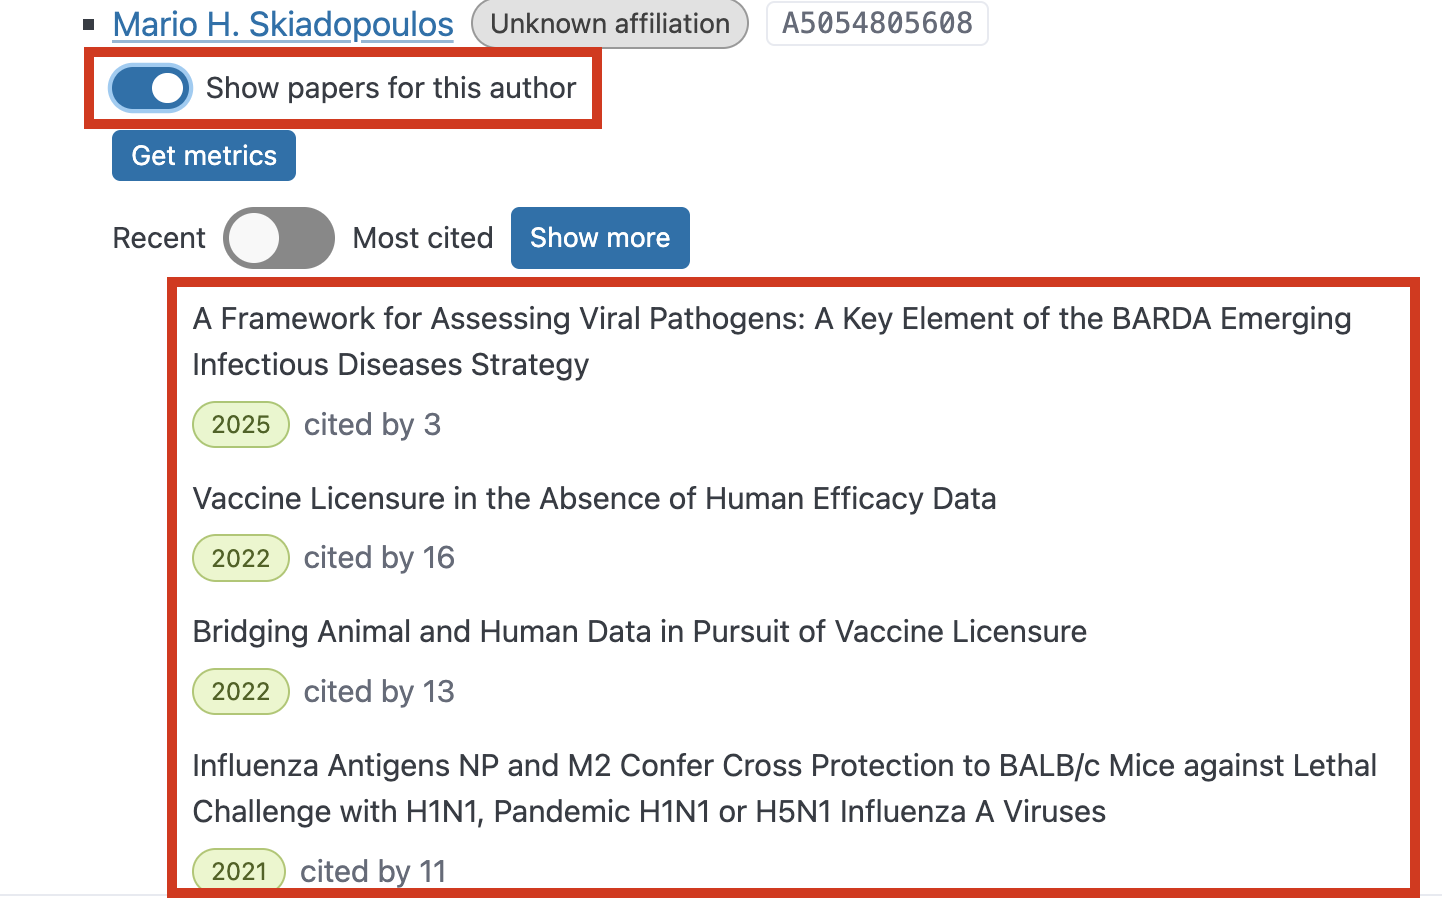
\includegraphics[scale=.4]{include/ui/search-res-5.3}
    \caption{Showing the papers of an author without an affiliation}
    \label{fig:ui-individual-papers}
\end{figure}

Figure~\ref{fig:ui-paper-order} shows the two ways of ordering the papers of the same author.
The list initially shows five papers, ordered by the publication date (\emph{most recent} first), with an option to order by citation count (\emph{most cited} first).
The \emph{Show more} button allows to load the rest of the list, beyond the initially shown five papers.

\begin{figure}[tb]
    \centering
    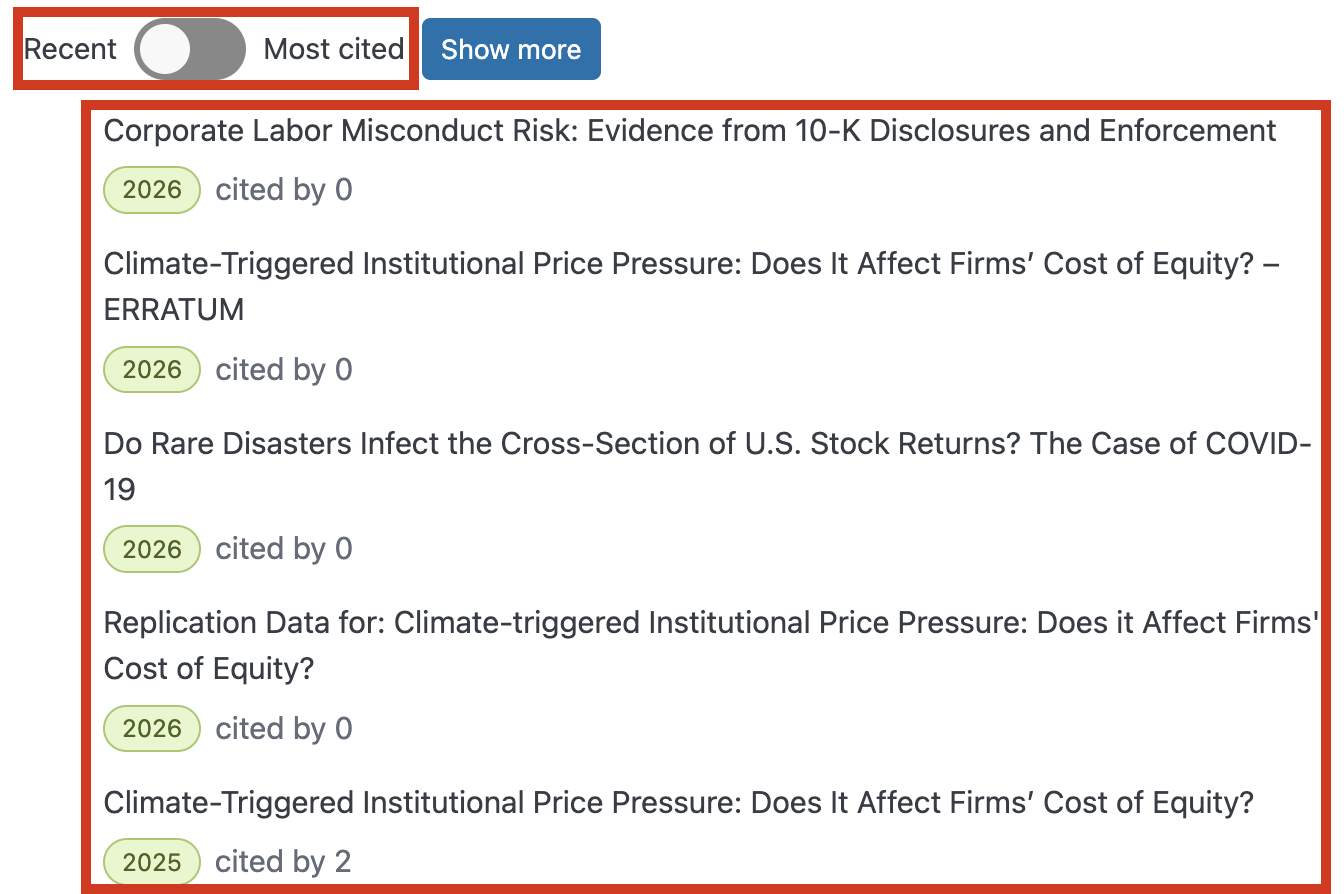
\includegraphics[scale=.3]{include/ui/search-res-5.1}
    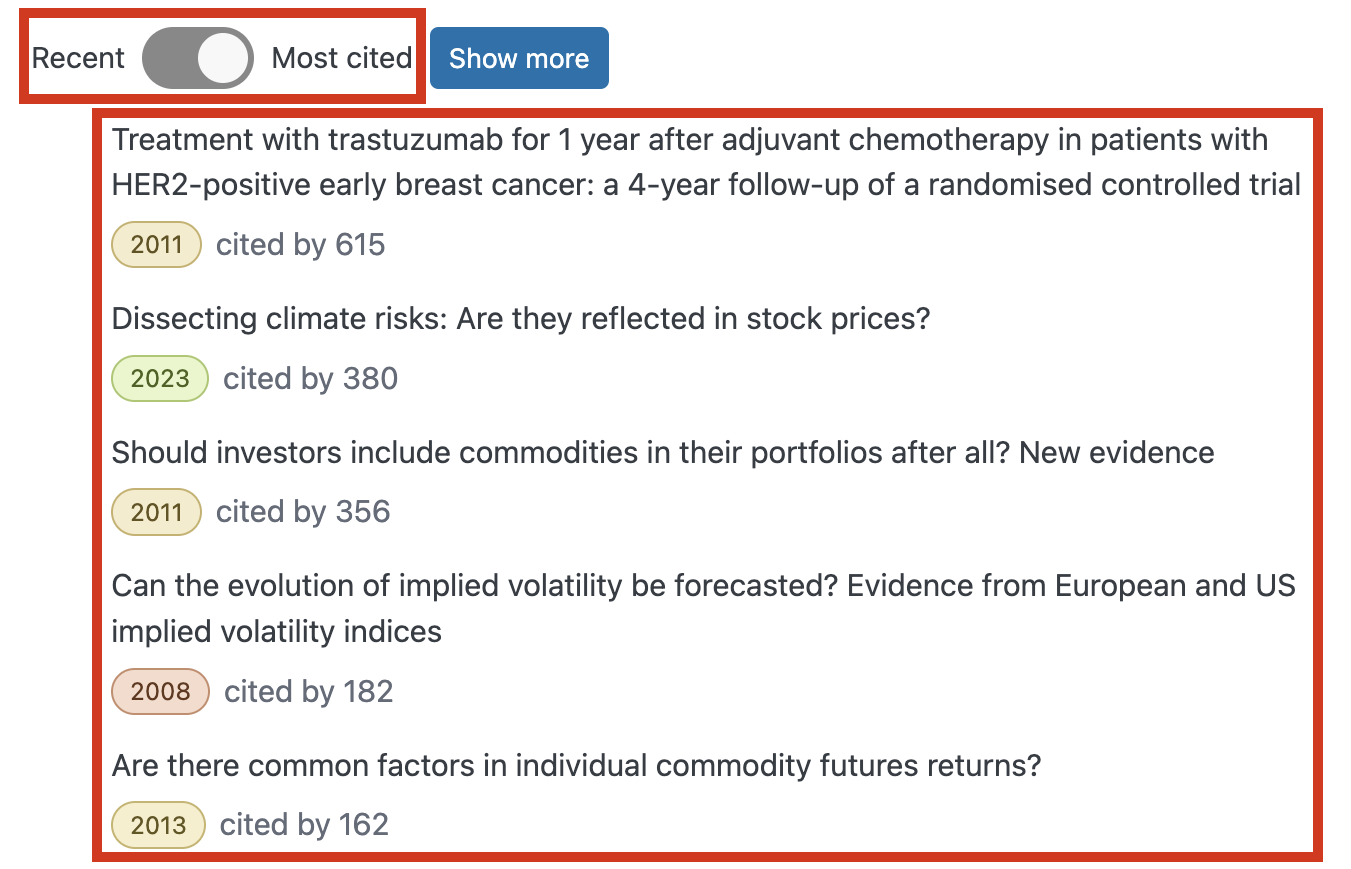
\includegraphics[scale=.3]{include/ui/search-res-5.2}
    \caption{Papers ordered most recent or most cited first}
    \label{fig:ui-paper-order}
\end{figure}

Users must explicitly request publication lists to be shown, to avoid unnecessary provider requests when the author is already recognizable.

Figure~\ref{fig:ui-get-metrics} shows the button \emph{Get metrics} that is available for every author, the user can click to request the citation metrics, starting the job as described in Section~\ref{sec:processing-pipeline}.

\begin{figure}[tb]
    \centering
    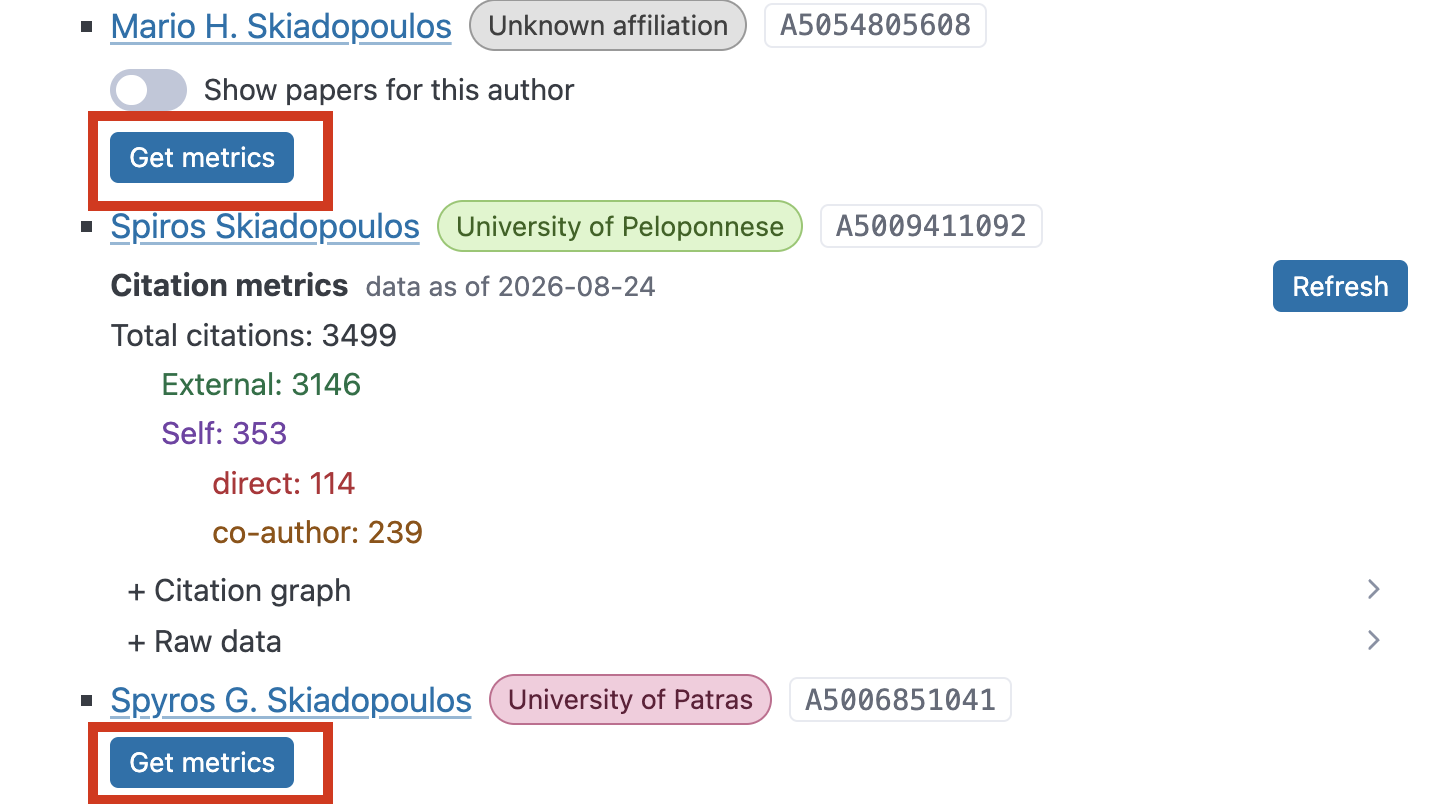
\includegraphics[scale=.4]{include/ui/search-res-6}
    \caption{Requesting citation metrics for an author}
    \label{fig:ui-get-metrics}
\end{figure}

Figure~\ref{fig:ui-metrics-progress} shows the progress under the selected author name, with the number of requests \textsf{completed}, \textsf{queued} and \textsf{failed}, updated while the job is running.

\begin{figure}[tb]
    \centering
    
\includegraphics[scale=.4]{include/ui/search-form-2}
    \caption{Progress while collecting the selected author's citations}
    \label{fig:ui-metrics-progress}
\end{figure}

Figure~\ref{fig:ui-metrics} shows the completed citation breakdown.
The completed result returns the breakdown of the number of citations, with counts for: \textsf{total}, \textsf{external}, and \textsf{direct} and \textsf{co-author} self-citations.

\begin{figure}[tb]
    \centering
    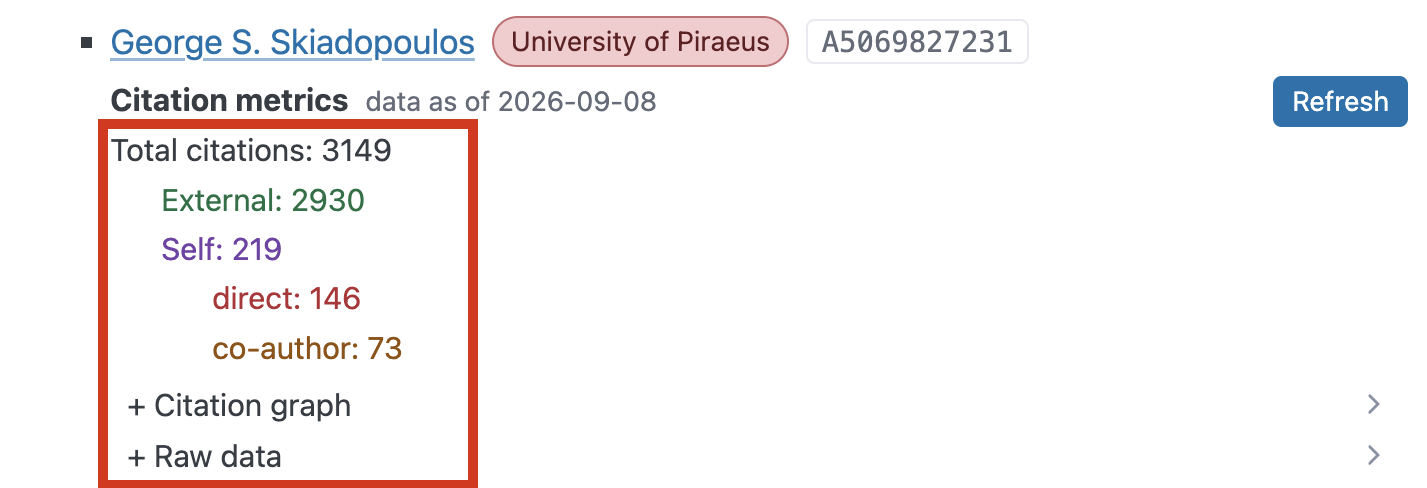
\includegraphics[scale=.4]{include/ui/search-res-7}
    \caption{The citation breakdown in the search results}
    \label{fig:ui-metrics}
\end{figure}

Counts summarize the result, but to provide more detailed information and a graph visualization, there are two initially collapsed options at the bottom of an author section.

Figure~\ref{fig:ui-graph} shows the graph chart, opened by clicking the \emph{Citation graph} link.
It represents the selected author, their own papers and the citing papers.

\begin{figure}[tb]
    \centering
    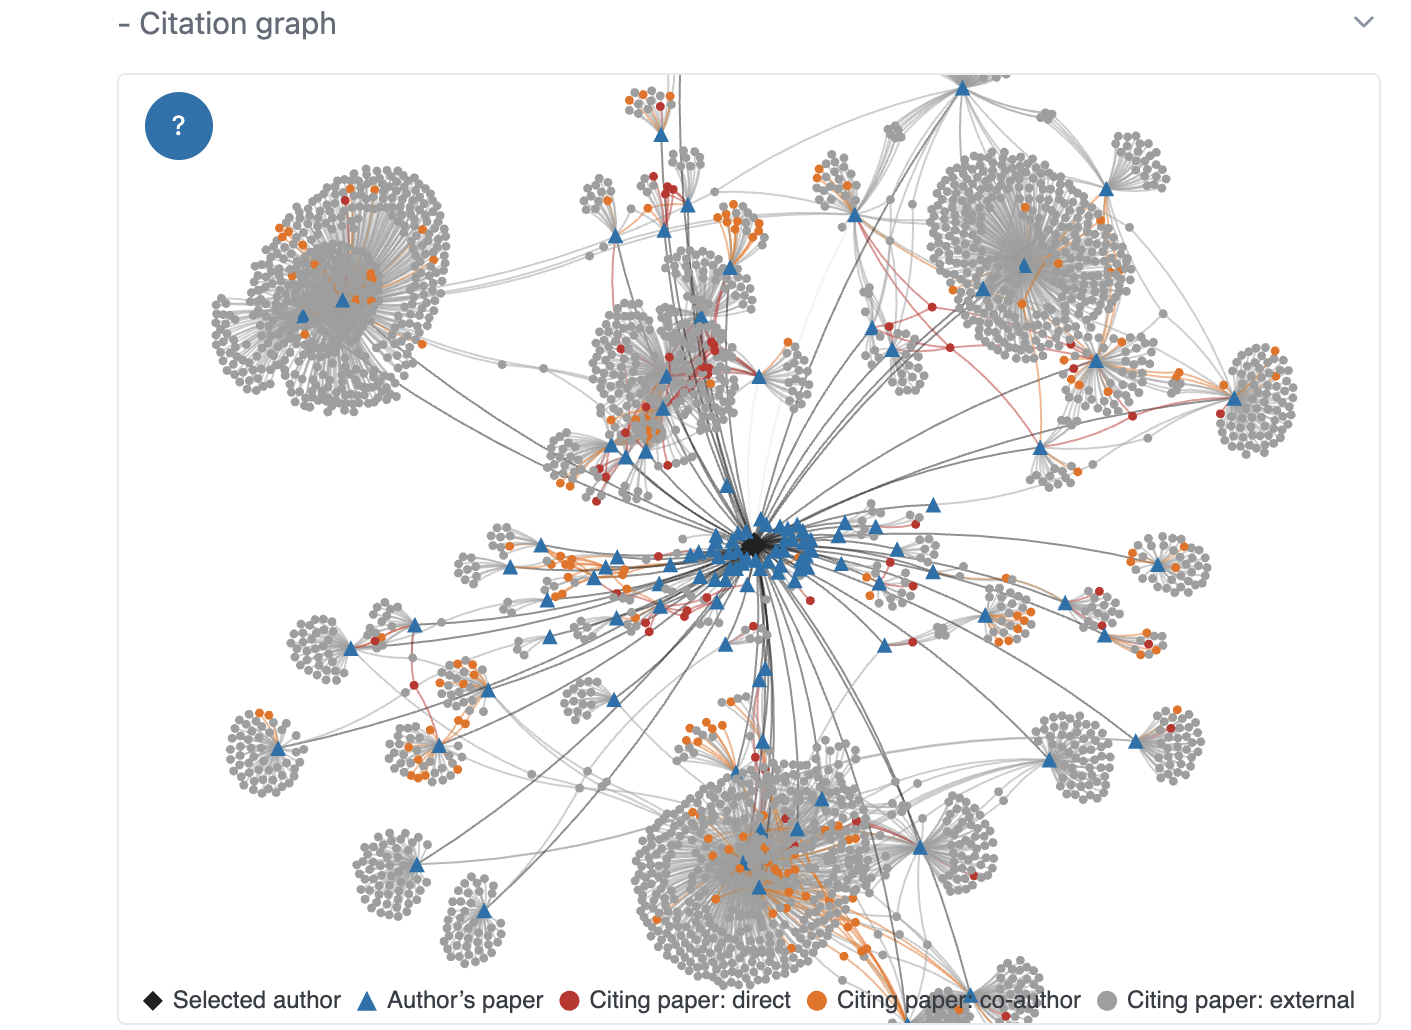
\includegraphics[scale=.4]{include/ui/author-details-2}
    \caption{The expanded citation graph}
    \label{fig:ui-graph}
\end{figure}

The connecting lines (graph edges) represent the relations between the selected author and their papers (\textsf{contribution}), and the selected author papers and citing papers (\textsf{citation}).

The graph supports zooming and panning, and hovering over a node reveals its details.

Figure~\ref{fig:ui-graph-filter} shows the graph filtered by excluding one of the node types.
There is a legend at the bottom of the chart explaining the shapes and colors of the graph, and acting as a filter, to hide or show the respective nodes by clicking on each category.
The citing papers are colored by the classification (\textsf{direct}, \textsf{co-author}, \textsf{external}).
A large graph is difficult to inspect with every citation visible; in the figure, the external citations are hidden, which leaves only the self-citations rendered in the graph.

\begin{figure}[tb]
    \centering
    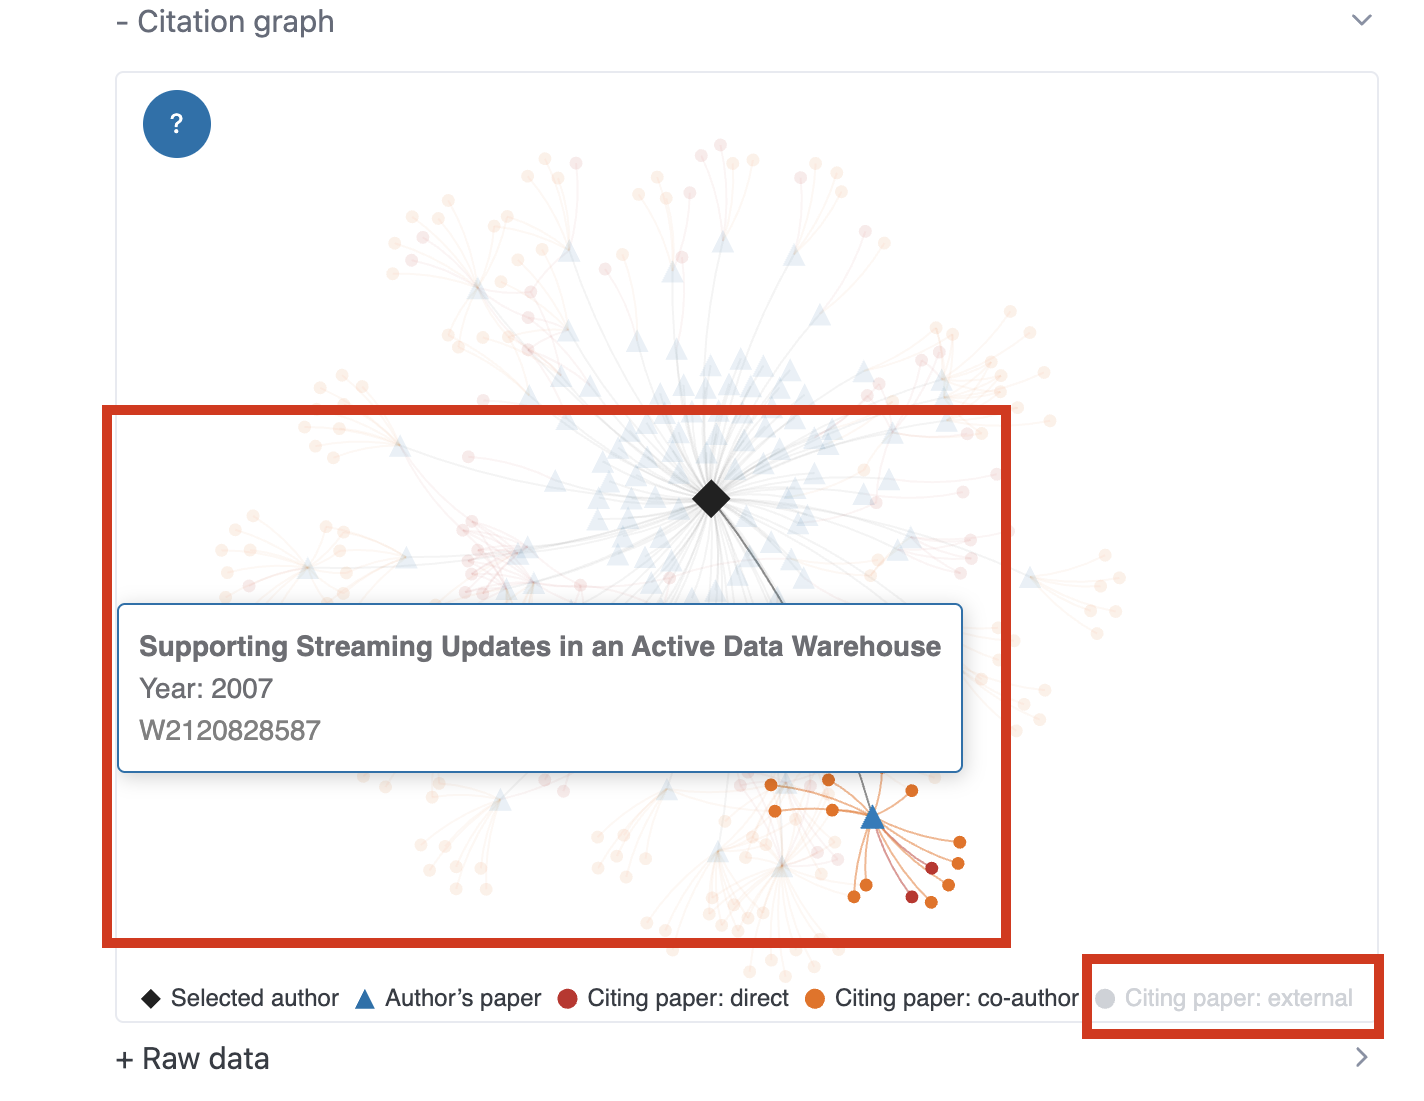
\includegraphics[scale=.4]{include/ui/author-details-5}
    \caption{Publication details with external citations hidden}
    \label{fig:ui-graph-filter}
\end{figure}

\subsection{Author details} \label{sec:ui-details}

\begin{figure}[tb]
    \centering
    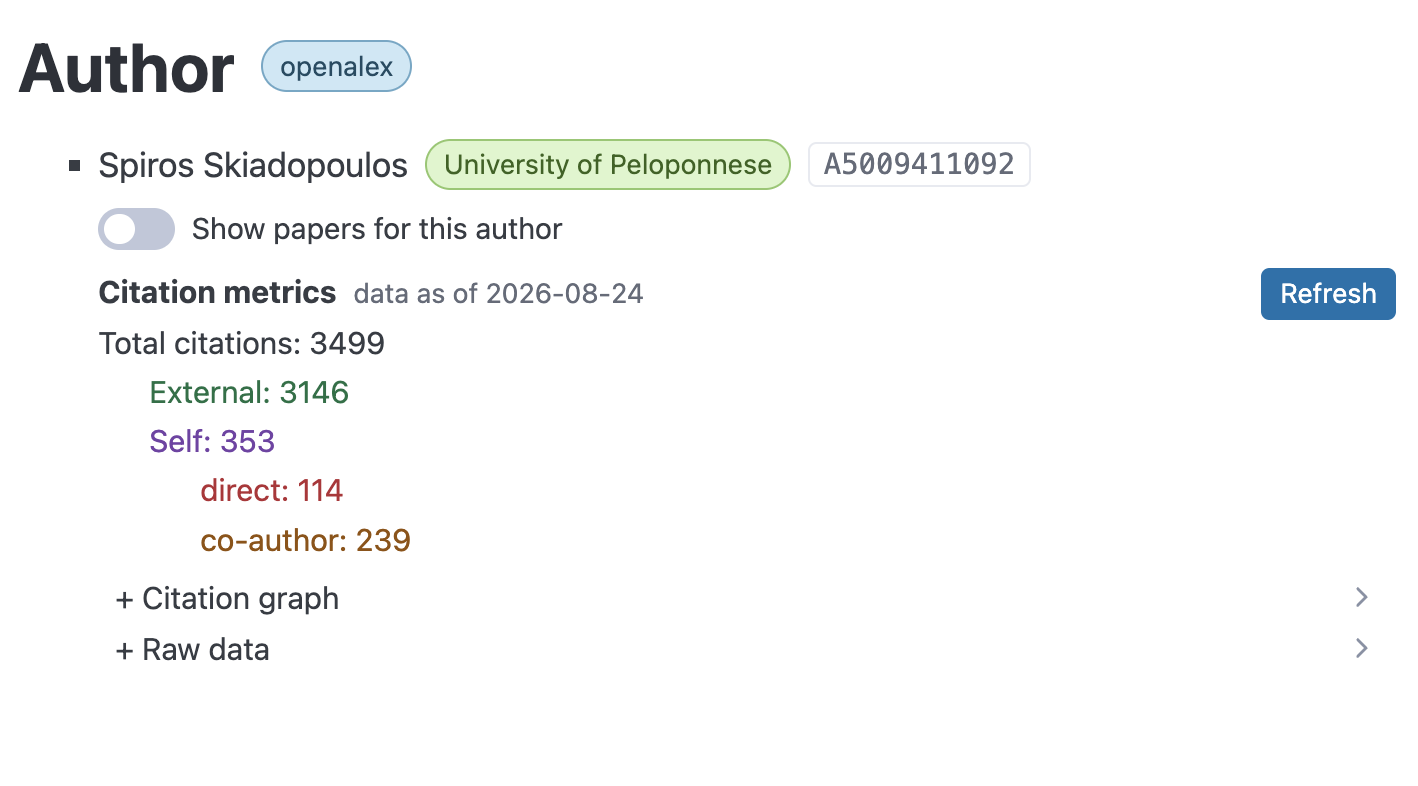
\includegraphics[scale=.4]{include/ui/author-details-1}
    \caption{A separate page for the selected author}
    \label{fig:ui-author}
\end{figure}

Figure~\ref{fig:ui-author} shows the page for the selected author, that can be opened by clicking on an author name.
As any other link, it can be opened in a new browser tab, allowing multiple author results to be open side by side.

The author name, the provider and the affiliation are rendered in the header of the page.
The remaining space on the page is occupied by the controls identical to the structure of the individual author details shown in the search results, as described in Section~\ref{sec:ui-results}.

\subsection{Status} \label{sec:ui-status}

Figure~\ref{fig:ui-status} shows the provider and system details panel.
Normally, it stays collapsed at the bottom of the page.
Clicking the \emph{Show status} button opens the panel, showing the request rate limit (requests per second), quotas, and the number of stored records for each provider, as well as jobs.
API keys are shown masked, only to identify that an API key is used, which can be helpful for providers that allow access with or without an API key, for instance \textsf{Semantic Scholar}.

The application version, together with the system resources (including the available memory and disk space) appear below the table.
These details are useful when investigating service disruptions.

\begin{figure}[tb]
    \centering
    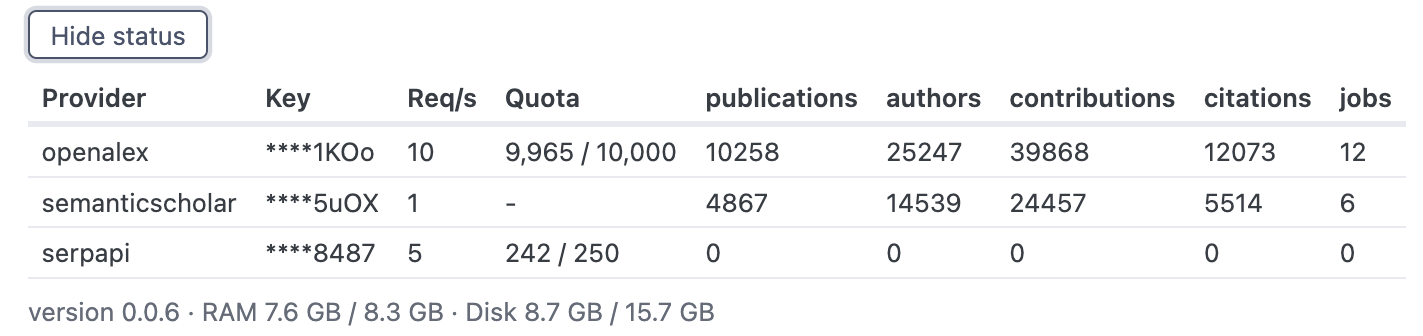
\includegraphics[scale=.4]{include/ui/status-1}
    \caption{Provider and system status}
    \label{fig:ui-status}
\end{figure}

\section{Testing} \label{sec:testing}

The backend, as the subsystem containing all business logic, is covered by automated tests, validating the outputs of all units of each component in isolation (such as services, repositories, connectors, controllers).
The unit tests guarantee that the behavior of each unit remains within the expectations.

The tests are written with \textsf{Jest}\footnote{\url{https://jestjs.io}} - one of the popular JavaScript unit test libraries.
Tests are organized into suites, where each suite covers the behavior of a single component.

The tests never touch real databases, the clock or the network.
Instead, every dependency of the unit under test is replaced by a mock fixture, allowing to program the expected results on each invocation.

This approach is convenient to make the unsuccessful paths reproducible.
By mocking the dependencies, unit tests can simulate all paths of behavior of an external provider: successful or erroneous responses, malformed data, empty results and so on.

The tests are placed near the components they cover, in \textsf{\_\_tests\_\_} directories at the same file system level.

On every push to the repository, a workflow executed by a \textsf{GitHub Actions} runner invokes the unit tests, and if any one of these fails, the pipeline exits with an error.
This mechanism prevents building and deploying versions of the application with invalid logic.

The unit tests follow a convenient nested structure, allowing to cover every branch of the source code logic.
Each level explores a scenario, by progressively refining the circumstances, to finally get to the inner blocks starting with \emph{it}, which performs a single call and asserts an outcome expectation.

Listing~\ref{lst:retry-tests} shows the outlined version of the suite testing \textsf{RetryStrategy}, the component responsible for retrying failed requests.
The method \textsf{run} executes the target function, and if the outcome is deemed retriable, it repeats the call, to either reach a successful outcome or exhaust the maximum allowed number of retries.

\begin{lstlisting}[float=tb, language=Java, caption={Structure of the retry strategy unit test suite}, label={lst:retry-tests}]
describe('RetryStrategy', () => {
  describe('run', () => {
    describe('when the function succeeds', () => {
      it('returns the value', ...);
      it('calls the function once', ...);
    });
    describe('when the function fails', () => {
      describe('but the error is not retryable', () => {
        it('does not retry', ...);
        it('passes the error to the retry check', ...);
      });
      describe('and the error is retryable', () => {
        describe('and a retry succeeds', () => {
          it('returns the eventual value', ...);
          it('stops calling once it succeeds', ...);
        });
        describe('but the retries are exhausted', () => {
          it('gives up with the error', ...);
          it('tries maxRetries + 1 times', ...);
        });
      });
    });
  });
});
\end{lstlisting}

Running the suite prints the titles of each branch and test, resulting in the same nested structure.
Listing~\ref{lst:retry-test-run} shows the output of the same retry strategy suite.

\begin{lstlisting}[float=tb, caption={Output of the retry strategy unit tests}, label={lst:retry-test-run}, literate={✓}{{\ensuremath\checkmark}}1]
PASS src/lib/__tests__/RetryStrategy.test.js
  RetryStrategy
    run
      when the function succeeds
        ✓ returns the value
        ✓ calls the function once
      when the function fails
        but the error is not retryable
          ✓ does not retry
          ✓ passes the error to the retry check
        and the error is retryable
          and a retry succeeds
            ✓ returns the eventual value
            ✓ stops calling once it succeeds
          but the retries are exhausted
            ✓ gives up with the error
            ✓ tries maxRetries + 1 times
\end{lstlisting}

\snote{Colors on Listing \ref{lst:retry-test-run}}

